\documentclass{article}
\usepackage{graphicx}
\usepackage{booktabs}
\usepackage{hyperref}
\usepackage[backend=biber, style=numeric, sorting=none]{biblatex}
\usepackage{amsmath}
\usepackage{multirow}
\usepackage{siunitx}
\usepackage[margin=1in]{geometry}

\graphicspath{ {./images/} }

\addbibresource{refs.bib}

\title{Systematic Hyperparameter Optimization and Benchmarking of Graph Neural Networks for ADMET Prediction}
\author{Martin, Mila, Adrian, Viktorija, Ilinka}
\date{\today}

\begin{document}

\maketitle

\begin{abstract}
This paper presents a comprehensive benchmarking framework for evaluating Graph Neural Networks (GNNs) on molecular property prediction, focusing on hyperparameter optimization (HPO) across six Absorption, Distribution, Metabolism, Excretion, and Toxicity (ADMET) datasets from the Therapeutics Data Commons (TDC). We systematically evaluated seven HPO algorithms---Random Search, Particle Swarm Optimization (PSO), Simulated Annealing (SA), Genetic Algorithm (GA), Artificial Bee Colony (ABC), Hill Climbing (HC), and Tree-structured Parzen Estimator (TPE)---conducting over 2,100 training runs. Our findings reveal that no single optimizer is universally superior; the optimal choice is task-dependent. Random Search proved to be a formidable baseline, outperforming more complex methods on several regression tasks. For classification, metaheuristics such as SA and ABC achieved the strongest performance. The study highlights the variable difficulty of ADMET tasks: GNNs achieved strong performance on toxicity prediction (hERG AUC-ROC: 0.825), but struggled with complex pharmacokinetics such as hepatocyte clearance, where the model performed worse than a mean baseline ($R^2 = -1.019$). We also demonstrate that scaffold-based splitting poses a critical challenge for foundation models, exposing severe overfitting in ChemBERTa (validation AUC of 0.82 vs.\ test AUC of 0.46 on Tox21). The paper provides a detailed overview of the benchmarking methodology, an in-depth analysis of the results, and practical recommendations for researchers in the field.
\end{abstract}


\section{Introduction}

Machine learning methods have become increasingly valuable in drug discovery, offering the potential to accelerate the identification and optimization of therapeutic candidates. Deep learning models, in particular, have been applied to a wide range of molecular property prediction tasks, leveraging architectures specialized for different data modalities including text, images, and graphs. Among these, Graph Neural Networks (GNNs) have emerged as a natural fit for molecular data, as they operate directly on molecular graph representations where atoms serve as nodes and bonds as edges.

Despite rapid progress in molecular machine learning, reported performance often depends heavily on the evaluation protocol. In particular, scaffold-based splitting (using Bemis--Murcko scaffolds~\cite{moleculenet}) creates a more realistic generalization setting by separating compounds with different core structures, but it also induces a strong distribution shift. As a result, models that perform well under random splits can degrade substantially under scaffold splits, especially for chemically diverse ADMET endpoints. This motivates systematic, reproducible benchmarking under scaffold-split evaluation to avoid overly optimistic conclusions.

To conduct such a benchmark, one requires well-curated datasets suitable for both training and cross-model comparison. The Therapeutics Data Commons (TDC)~\cite{tdc} provides a comprehensive collection of Absorption, Distribution, Metabolism, Excretion, and Toxicity (ADMET) datasets covering how molecules are absorbed, distributed, metabolized, and excreted by the body, as well as their toxicity across various biological assays.

In addition to providing datasets with standard splits, TDC maintains leaderboards of top-performing models along with their results, some of which are discussed in the following section. These leaderboards, together with community-organized challenges, facilitate direct comparison of approaches and drive progress in the field.

In this work, we present a reproducible benchmarking framework for molecular property prediction that systematically evaluates HPO strategies for GNNs across six TDC ADMET tasks. Unlike prior work focused on proposing new molecular architectures, our study centers on evaluation methodology and optimization behavior under controlled experimental settings, enabling reproducible comparisons across datasets and HPO strategies.

The study includes seven HPO algorithms with 50 trials per dataset--algorithm combination (2,100+ total model evaluations), a comparison against multiple foundation-model baselines (ChemBERTa~\cite{chemberta2}, MolCLR~\cite{molecularConstrastive}, Morgan fingerprints, MolE-style learned fingerprints~\cite{MolE}), and multi-seed validation to quantify statistical robustness.

\noindent\textbf{Contributions.} We make the following contributions:
\begin{itemize}
    \item We benchmark \textbf{seven HPO algorithms} (Random, PSO, ABC, GA, SA, HC, TPE) on \textbf{six ADMET datasets} from TDC under a consistent scaffold-split evaluation protocol.
    \item We run \textbf{50 trials} per algorithm--dataset pair, totaling \textbf{2,100+ training runs}, and analyze optimization behavior and budget efficiency.
    \item We provide \textbf{multi-seed validation} (5 seeds) with confidence intervals to assess result stability and reproducibility.
    \item We compare optimized GNNs against \textbf{foundation model baselines} and document the severe scaffold-split sensitivity of SMILES-based transformers.
    \item We derive \textbf{practical recommendations} on which HPO strategy to use for various molecular prediction tasks under limited compute budgets.
\end{itemize}


\section{Related Work}

The TDC ADMET Leaderboards feature a wide range of machine learning models designed for molecular property prediction. Notably, some of the strongest results come from relatively simple approaches. For example, MapLight~\cite{maplight} combines random forests and SVMs with molecular node embeddings, achieving competitive performance. For certain datasets, classical methods such as Random Forest and XGBoost have yielded top results, motivating ensemble strategies such as FCA~\cite{fca}, which constructs a weighted combination of multiple models.

Our primary focus, however, is on deep learning approaches. Among the simplest yet effective architectures is AttentiveFP~\cite{attentiveFP}, which combines Graph Convolutional Network (GCN) and Graph Attention Network (GAT) layers with Gated Recurrent Unit (GRU) layers. AttentiveFP achieves top-5 results across multiple datasets, in part due to its integration of both edge and node features at the input stage.

More advanced deep learning approaches borrow techniques from large language models. These include attribute masking~\cite{attrMasking} and contrastive learning~\cite{molecularConstrastive}. Masking involves removing certain node or edge attributes and training the model to predict the missing values, thereby learning robust molecular embeddings. Contrastive learning is a more general self-supervised technique in which augmented views of the same molecular graph are trained to produce similar embeddings, while embeddings from different molecules are pushed apart.

Both masking and contrastive learning are commonly used in molecular foundation models. These models typically follow a multi-stage pipeline: first learning molecular embeddings through self-supervised pretraining, then training on multiple prediction tasks simultaneously, and finally fine-tuning for a specific target property. Examples include DeepMol~\cite{deepMol} and MolE~\cite{MolE}. A distinct approach is taken by ChemBERTa~\cite{chemberta2}, which applies a RoBERTa-based language model to learn embeddings from SMILES strings rather than operating directly on molecular graphs. A notable drawback of such foundation models is their large size, which makes them both more expensive to train and less practical for deployment in resource-constrained settings.

Recent work has highlighted that transformer-based models exhibit severe distribution shift when evaluated on scaffold-split datasets, achieving high validation AUC but near-random test performance. Our experiments confirm this finding, with ChemBERTa achieving a validation AUC of 0.82 but a test AUC of only 0.46 on Tox21.

\subsection{Hyperparameter Optimization for Molecular ML}
Hyperparameter optimization is a key driver of performance in deep learning and is particularly important in molecular property prediction, where datasets are typically small and noisy. Random Search is a strong baseline that can outperform grid search by exploring more diverse configurations when only a subset of hyperparameters is influential~\cite{bergstra2012random}. Bayesian optimization methods such as the Tree-structured Parzen Estimator (TPE), implemented in frameworks like Optuna~\cite{optuna}, model the relationship between hyperparameters and validation performance to improve sample efficiency. In molecular ML, where each training run can be costly, TPE-style methods are often attractive under limited trial budgets. In contrast, population-based metaheuristics (PSO, GA, ABC) provide broader exploration of the search space but may require larger budgets to converge reliably.

\subsection{Foundation Models and Molecular Representation Learning}
Recent foundation models for chemistry include SMILES-based transformers (e.g., ChemBERTa~\cite{chemberta2}) and graph-based contrastive methods (e.g., MolCLR~\cite{molecularConstrastive}). While pretrained representations can transfer across tasks, their effectiveness depends on the evaluation protocol. In particular, scaffold-split evaluation can expose distribution shifts that lead to strong validation performance but poor test-set generalization for models that overfit to chemical substructures or tokenization patterns. This motivates comparing task-specific end-to-end GNN training with pretrained encoders used as frozen feature extractors or with limited fine-tuning.


\section{Materials and Methods}

\subsection{Datasets and Evaluation Protocol}
We evaluate on six ADMET datasets using scaffold-based splitting (Bemis--Murcko scaffolds~\cite{moleculenet})
with an 80/10/10 train/validation/test ratio and a fixed seed (42) for reproducibility.
During HPO, the test split remains fully held out; model selection is performed solely
on the validation metric, and final performance is reported once on the test split.

\paragraph{Splitting protocol.}
We use the TDC two-way scaffold split and manually subdivide the resulting training portion
into 90/10 train/validation subsets. This ensures that molecules with different core structures
are separated across splits, better reflecting real-world generalization to novel chemical space.

\paragraph{Target transformations.}
For regression tasks, we apply log transformation for skewed target distributions and clip targets
to a minimum value of $10^{-3}$ for non-Caco2 datasets, followed by standardization using the
train+validation statistics. For classification tasks, targets are binary encoded and we apply
class weighting to mitigate severe imbalance (e.g., Tox21 NR-AR).


\subsection{Optimization Algorithms}
\subsubsection{Genetic Algorithm}
\textbf{Genetic Algorithms} (GAs) draw inspiration from natural selection and evolutionary principles, advancing a population of candidate solutions through multiple generations. Each candidate encodes a potential hyperparameter configuration, typically represented as a chromosome. The population evolves through biologically inspired operations---selection, crossover, and mutation---that progressively improve fitness as measured by model performance metrics. For hyperparameter tuning, GAs excel at navigating complex, high-dimensional search spaces by effectively balancing exploration of new regions with exploitation of promising areas. The mutation and recombination mechanisms prove particularly valuable for escaping local optima, making GAs well-suited for non-convex and discrete hyperparameter landscapes.
\subsubsection{Particle Swarm Optimization}
\textbf{Particle Swarm Optimization} (PSO) abstracts the collective behavior of bird flocks and schooling fish to solve continuous optimization problems. Each particle represents a candidate hyperparameter configuration and iteratively updates its position by considering both its own historical best performance and the best solution discovered by the entire swarm. This combination of individual and collective learning creates an effective balance between exploratory and exploitative search, allowing PSO to converge efficiently toward high-quality hyperparameter sets. PSO is particularly effective for continuous and real-valued hyperparameters, offering the dual advantages of straightforward implementation and minimal hyperparameter tuning requirements for the optimizer itself.
\subsubsection{Artificial Bee Colony}
\textbf{Artificial Bee Colony} (ABC) optimization mimics the foraging behavior of honeybee colonies. The algorithm maintains three bee types---employed bees, onlookers, and scouts---each contributing distinct exploration and exploitation capabilities. Candidate solutions are treated as nectar sources, and bees collaboratively search nearby solutions, assess their quality, and disseminate information throughout the colony. The ABC algorithm dynamically equilibrates exploration and exploitation, achieving robust performance across both discrete and continuous hyperparameter spaces.
\subsubsection{Hill Climbing}
\textbf{Hill Climbing} (HC) is one of the simplest optimization heuristics. Starting from an initial hyperparameter configuration, the algorithm transitions to a neighboring configuration only when it yields improved model performance. This greedy approach enables fast convergence in smooth, unimodal search landscapes but is vulnerable to premature convergence at local optima, particularly in the non-convex hyperparameter spaces common in deep learning. Despite this limitation, Hill Climbing remains practical when the hyperparameter space is limited in dimensionality or when adequate initialization strategies are available.
\subsubsection{Random Search}
\textbf{Random Search} is a widely used baseline for hyperparameter optimization, operating by uniformly sampling configurations across the search space~\cite{bergstra2012random}. This method proves particularly valuable in high-dimensional optimization problems where only a limited subset of hyperparameters meaningfully influences performance. Research has demonstrated that Random Search frequently surpasses grid search when the search space contains non-critical hyperparameters, as it allocates resources more effectively by exploring diverse configurations instead of exhaustively examining irrelevant parameter combinations. Its main advantages are simplicity, ease of parallelization, and the absence of assumptions about search space structure.
\subsubsection{Simulated Annealing}
\textbf{Simulated Annealing} (SA) adapts the physical annealing process used in metallurgy to optimization problems. The algorithm explores the solution space while accepting both improvements and strategically worse solutions with a probability that decreases over time, helping to escape local optima. When applied to hyperparameter optimization, SA initiates with an initial configuration and iteratively generates neighboring candidates through controlled perturbations. As the temperature gradually decreases, the algorithm transitions toward a more conservative mode, concentrating optimization efforts around the best configurations identified throughout the search.
\subsubsection{Tree-structured Parzen Estimator}
\textbf{Tree-structured Parzen Estimator} (TPE) is a Bayesian optimization method implemented via the Optuna framework~\cite{optuna}. Unlike the metaheuristic algorithms above, TPE builds a probabilistic model of the objective function and uses it to select promising hyperparameter configurations, achieving better sample efficiency under limited budgets.

\subsection{Foundation Model Baselines}
We evaluate several representation-learning baselines to contextualize the optimized GNN performance: (i)~Morgan fingerprints (ECFP4) with an MLP predictor, (ii)~ChemBERTa~\cite{chemberta2} as a SMILES transformer encoder, (iii)~MolCLR-style contrastive graph embeddings~\cite{molecularConstrastive}, and (iv)~MolE molecular foundation model embeddings~\cite{MolE}. We consider two settings for pretrained encoders: \textbf{frozen encoder + trainable MLP head} and \textbf{limited fine-tuning} (ChemBERTa-FT) where we fine-tune the encoder with a small learning-rate sweep while keeping the downstream head fixed.

For the frozen setting, embeddings are extracted once per molecule and an MLP is trained on the train split, with early stopping based on the validation split. For fairness under compute constraints, baselines use a fixed head architecture and a small learning-rate sweep, while the GNN receives the full 50-trial HPO budget. All baselines use the same dataset splits and evaluation metrics as the GNN experiments.


\subsection{Benchmarking Framework Overview}
The benchmarking framework provides a systematic infrastructure for evaluating, comparing, and optimizing GNNs and foundation models for molecular property prediction across ADME and toxicity tasks. It enables researchers to identify performance bottlenecks, validate architectural and hyperparameter choices, and ensure that predictive models meet accuracy requirements across diverse molecular datasets. Figure~\ref{fig:benchmark-framework} illustrates the overall architecture.

\subsubsection{Architectural Design and Components}
At the core of this framework lies a modular architecture ensuring flexibility and extensibility, qualities essential for machine learning research where model architectures, evaluation protocols, and performance metrics evolve continuously. The framework comprises five fundamental components, each fulfilling a distinct yet synergistic role:

\textbf{The Benchmark Manager} orchestrates the entire evaluation process, coordinating execution of multiple model configurations across six molecular datasets (four ADME regression tasks and two toxicity classification tasks), managing experimental configurations specifying architectural choices and hyperparameters, and ensuring consistent evaluation protocols enabling fair comparisons between different optimization strategies.

\textbf{The Metrics Collector} implements a multi-faceted measurement system capturing performance indicators across prediction quality, computational efficiency, and training dynamics. This component employs a plugin-based architecture where specialized metric calculators operate independently, enabling seamless integration of novel evaluation criteria such as uncertainty quantification metrics or chemical space coverage assessments without requiring modifications to the core infrastructure.

\textbf{The Data Recorder} embodies separation between measurement and persistence by decoupling performance metric collection from storage implementation, supporting multiple backend options including CSV/JSON files for immediate inspection, structured databases for complex querying, and cloud storage for collaborative research environments.

\textbf{The Results Analyzer} provides comprehensive statistical analysis extending beyond simple metric aggregation to include cross-validation statistics with confidence intervals, statistical significance testing through Wilcoxon signed-rank tests, performance stratification across molecular subpopulations, and trend analysis revealing how model performance correlates with dataset characteristics such as molecular complexity or structural diversity.

\textbf{The Report Generator} transforms numerical results and statistical analyses into publication-ready outputs including comprehensive performance tables, architectural comparison visualizations, ablation study summaries, and methodology documentation.

\begin{figure}[t]
    \centering
    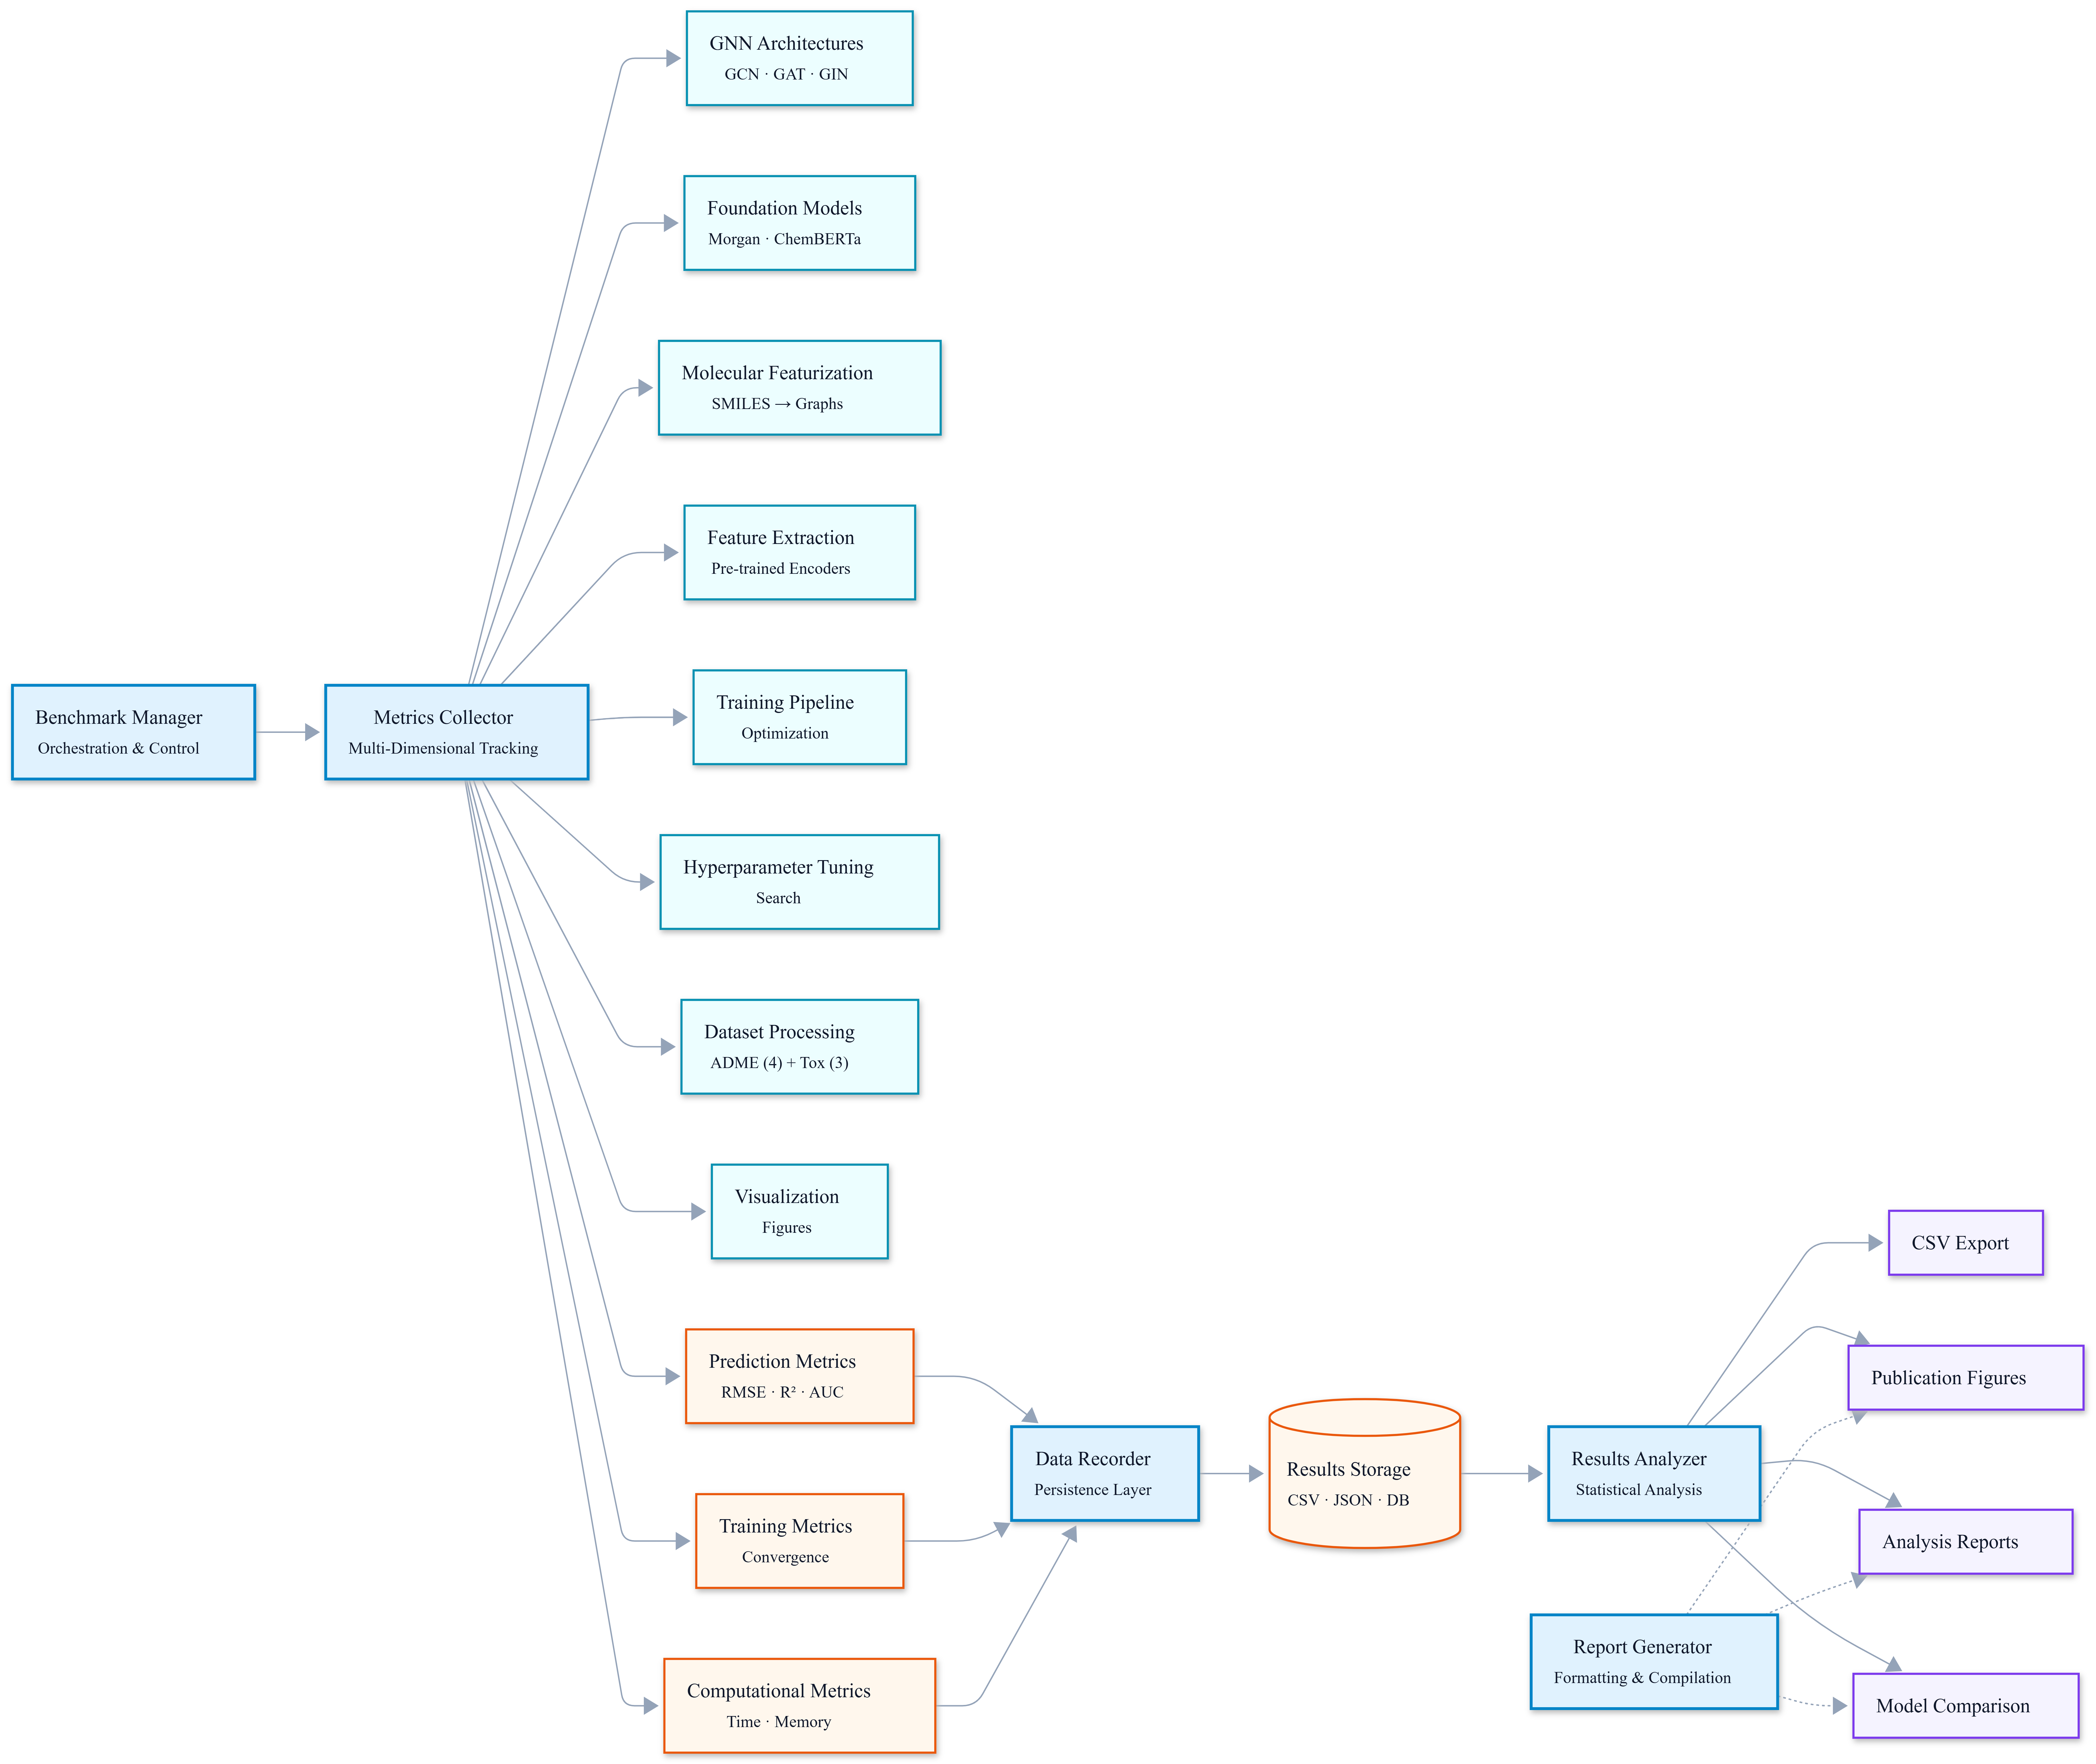
\includegraphics[width=\linewidth]{Benchmark-Architecture-GNN.png}
    \caption{Overview of the benchmarking framework for evaluating and optimizing molecular GNN and foundation models on ADMET tasks. The diagram depicts the high-level system components; individual module implementations may differ from the labels shown (e.g., the GNN encoder uses GraphConv layers rather than the GCN/GAT/GIN variants listed).}
    \label{fig:benchmark-framework}
\end{figure}

\subsubsection{Multi-Dimensional Performance Evaluation}
The framework's metrics collection operates across three interconnected dimensions characterizing model performance from complementary perspectives:

\begin{itemize}
    \item \textbf{Prediction Metrics} quantify molecular property prediction quality through:
    \begin{itemize}
        \item \textbf{Regression Metrics (ADME):} Root Mean Squared Error (RMSE) measuring average prediction deviation, coefficient of determination ($R^2$) indicating explained variance, and Mean Absolute Error (MAE) providing interpretable error magnitudes.
        \item \textbf{Classification Metrics (Toxicity):} Area Under the ROC Curve (AUC) measuring discrimination capability, Accuracy, and F1-score for balanced assessment of toxic/non-toxic predictions.
    \end{itemize}

    \item \textbf{Training Metrics} illuminate learning dynamics and optimization characteristics by tracking:
    \begin{itemize}
        \item Convergence speed measured through epochs required to reach performance plateaus
        \item Training stability quantified by loss curve variance and gradient statistics
        \item Generalization gap calculated as discrepancy between training and validation performance
        \item Overfitting indicators such as divergence between training and test set metrics
    \end{itemize}
    This temporal dimension reveals whether architectures learn efficiently from limited molecular data---crucial given that high-quality ADMET datasets typically contain only hundreds to low thousands of compounds.

    \item \textbf{Computational Metrics} measure:
    \begin{itemize}
        \item Wall-clock training time for full model optimization
        \item Inference latency for individual molecular predictions
        \item Memory consumption during forward and backward passes
        \item Parameter efficiency expressed as the ratio of model parameters to achievable performance
    \end{itemize}
    These metrics enable informed trade-offs between predictive accuracy and computational cost.
\end{itemize}

\subsubsection{Integration with GNN and Foundation Model Pipelines}

The framework integrates with both \textbf{GNN-based} and \textbf{foundation model-based} pipelines, each requiring specialized benchmarking approaches:

\begin{itemize}
    \item \textbf{GNN Model Architecture:} The framework evaluates a GraphConv-based~\cite{pyg} graph neural network with batch normalization, ReLU activations, and concatenated mean/max pooling. It optimizes architectural hyperparameters such as layer depth, hidden channel dimensions, and MLP head dimensions while profiling molecular featurization (graph construction time from SMILES strings) and its impact on downstream performance.

    \item \textbf{Foundation Models:} The framework supports benchmarking of:
    \begin{itemize}
        \item Pre-trained molecular embeddings (e.g., ChemBERTa~\cite{chemberta2}, MolE~\cite{MolE})
        \item Fingerprint-based approaches (Morgan-FP)
        \item Contrastive graph embeddings (MolCLR~\cite{molecularConstrastive})
    \end{itemize}
    For these models, the pipeline optimizes projection dimension, downstream predictor architecture (MLP depth/width), and learning dynamics, freezing the pre-trained encoder to evaluate representation quality. Performance assessment focuses on embedding extraction efficiency and transfer learning effectiveness.
\end{itemize}

The training pipeline receives comprehensive monitoring covering batch processing efficiency, gradient computation performance, parameter update overhead, and optimization strategy effectiveness including learning rate schedules, weight decay regularization, and early stopping criteria. Hyperparameter optimization procedures are tracked through search space exploration coverage, convergence to optimal configurations, and statistical reliability of performance estimates derived from cross-validation.


\section{Experiments, Results and Discussion}
\label{sec:experiments}

\subsection{Experimental Setup}
\label{sec:experimental_setup}

\subsubsection{Datasets}

We evaluated our framework on six molecular property prediction tasks from the TDC ADMET benchmark~\cite{tdc}: four ADME regression tasks and two toxicity classification tasks. Table~\ref{tab:dataset_stats} summarizes the dataset characteristics.

\begin{table}[h]
\centering
\caption{Dataset statistics and evaluation metrics (TDC ADMET).}
\label{tab:dataset_stats}
\small
\begin{tabular}{lcccc}
\toprule
\textbf{Dataset} & \textbf{Task Type} & \textbf{Samples} & \textbf{Split} & \textbf{Primary Metric} \\
\midrule
\multicolumn{5}{l}{\emph{ADME Regression}} \\
\midrule
Caco2\_Wang & Permeability & 910 & Scaffold & RMSE \\
Half\_Life\_Obach & Pharmacokinetics & 667 & Scaffold & RMSE \\
Clearance\_Hepatocyte\_AZ & Metabolism & 1,213 & Scaffold & RMSE \\
Clearance\_Microsome\_AZ & Metabolism & 1,102 & Scaffold & RMSE \\
\midrule
\multicolumn{5}{l}{\emph{Toxicity Classification}} \\
\midrule
Tox21 (NR-AR) & Endocrine toxicity & 7,258 & Scaffold & AUC-ROC \\
hERG & Cardiotoxicity & 655 & Scaffold & AUC-ROC \\
\bottomrule
\end{tabular}

\noindent\textit{Note:} Tox21 (NR-AR) has a 3.5\% positive rate and hERG has a 31\% positive rate; total molecules across all datasets: 11{,}805.
\end{table}


\subsubsection{Model Architecture and Training}

\paragraph{Model Architecture.}
We use a graph neural network backbone based on stacked GraphConv layers~\cite{pyg} with batch normalization and ReLU activation. Each molecule is represented as a molecular graph constructed from SMILES using RDKit. Atom-level features include atomic number, degree, formal charge, hybridization, aromaticity, ring membership, hydrogen count, and atomic mass (8 features per atom). Additionally, graph-level ADME descriptors (e.g., molecular weight, LogP, TPSA) are computed and concatenated with the pooled node representations. The GNN encoder produces node embeddings that are aggregated into a graph-level representation using concatenated global mean and max pooling. The pooled representation is then passed to a three-layer MLP prediction head with batch normalization. This design provides a stable and efficient backbone for systematic benchmarking under limited data regimes.


\textbf{Training Configuration.} All models were trained with:
\begin{itemize}
    \item Optimizer: Adam~\cite{adam} with default parameters
    \item Batch size: 32
    \item Maximum epochs: 100 (regression), 50 (classification)
    \item Early stopping: patience of 12 epochs on validation loss
    \item Loss: MSE (regression), binary cross-entropy with logits (classification)
    \item Target normalization: standardized to zero mean, unit variance
    \item Evaluation batch size: 64
    \item Gradient clipping: max norm = 1.0
    \item Class weighting: positive class weighting for imbalanced classification tasks (e.g., Tox21)
\end{itemize}

\subsubsection{Hyperparameter Optimization}

\textbf{Search Space:}
\begin{itemize}
    \item Hidden dimensions: \{64, 96, 128, 192, 256, 384, 512\}
    \item Number of GraphConv layers: \{3, 4, 5, 6, 7\}
    \item Learning rate: $[10^{-4}, 10^{-2}]$ (log-uniform)
    \item Weight decay: $[10^{-6}, 10^{-2}]$ (log-uniform)
    \item MLP head dimensions: three layers with categorical presets (layer~1: \{128, 192, 256, 384, 512\}; layer~2: \{64, 96, 128, 192, 256\}; layer~3: \{32, 48, 64, 96, 128\}), sorted in monotonically decreasing order for stability
\end{itemize}

\textbf{Optimization Algorithms:} We compared seven HPO strategies:
\begin{enumerate}
    \item Particle Swarm Optimization (PSO): population = 16
    \item Simulated Annealing (SA): $T_0=50$, cooling $\alpha=0.99$
    \item Genetic Algorithm (GA): population = 16, mutation rate = 0.1
    \item Artificial Bee Colony (ABC): colony size = 16, limit = 50
    \item Hill Climbing (HC): greedy local search
    \item Random Search: uniform sampling
    \item Tree-structured Parzen Estimator (TPE): Optuna~\cite{optuna} with 10 startup random trials and median pruning
\end{enumerate}

We select the best configuration based on validation RMSE (regression) or validation AUC (classification) and evaluate once on the held-out test split.

\noindent\textbf{HPO settings.} All metaheuristic algorithms were implemented via the NiaPy library~\cite{niapy}. We use population size 16 for PSO/ABC/GA, SA with $T_0=50$ and cooling $\alpha=0.99$, and Optuna TPE with 10 startup random trials and median pruning. All methods share the same search space to ensure fair comparison.



\subsubsection{Implementation}

\textbf{Software:} Python $\ge$ 3.8, PyTorch $\ge$ 2.0, PyTorch Geometric~\cite{pyg} $\ge$ 2.3, RDKit $\ge$ 2022.9, PyTDC $\ge$ 1.0, NiaPy~\cite{niapy} $\ge$ 2.0, Optuna~\cite{optuna} $\ge$ 3.0, Transformers $\ge$ 4.30

\textbf{Hardware:}
\begin{itemize}
    \item CPU: Intel Core i7-8700K @ 3.70\,GHz
    \item RAM: 16.0\,GB
    \item GPU: NVIDIA GeForce RTX 3060
    \item Total experiment time: approximately 45 hours
\end{itemize}

\subsubsection{Multi-Seed Validation}
To quantify robustness, we retrain the selected best configuration per dataset across five random seeds. We report the mean and standard deviation of the test metric across seeds. This prevents conclusions based on a single favorable run and enables more reliable comparisons between HPO strategies.

\subsubsection{Statistical Significance Testing}
We compare HPO algorithms against Random Search using paired tests on the per-dataset results. For each comparison, we apply the Wilcoxon signed-rank test and additionally report effect sizes to capture practical significance beyond $p$-values.


\subsection{Results}
\label{results}
\subsubsection{Hyperparameter Optimization Performance}
\label{sec:hpo_performance}

We evaluated seven hyperparameter optimization algorithms across our benchmark of six ADME and toxicity prediction tasks. Table~\ref{tab:hpo_results} presents a comprehensive comparison of algorithm performance on regression and classification tasks, revealing notable differences in optimization efficiency and final model quality.
\subsubsection{TPE Benchmark (Optuna)}
\label{sec:tpe_benchmark}

Since TPE is implemented via Optuna and reported as a dedicated benchmark in our framework,
we summarize its standalone results separately for direct comparison with the best GNN runs.

\begin{table}[t]
\centering
\caption{TPE benchmark results from Optuna (test split). RMSE $\downarrow$ for regression, AUC-ROC $\uparrow$ for classification.}
\label{tab:tpe_results}
\small
\begin{tabular}{lcc}
\toprule
\textbf{Dataset} & \textbf{Task} & \textbf{TPE Result} \\
\midrule
Caco2\_Wang & RMSE $\downarrow$ & 0.0030 \\
Half\_Life\_Obach & RMSE $\downarrow$ & 22.34 \\
Clearance\_Hepatocyte\_AZ & RMSE $\downarrow$ & 52.16 \\
Clearance\_Microsome\_AZ & RMSE $\downarrow$ & 44.34 \\
Tox21 (NR-AR) & AUC-ROC $\uparrow$ & 0.705 \\
hERG & AUC-ROC $\uparrow$ & 0.772 \\
\bottomrule
\end{tabular}
\end{table}

\begin{table}[t]
\centering
\caption{HPO algorithm comparison across datasets within a 50-trial budget. Values show test metrics for each optimizer. Best per dataset in \textbf{bold}. TPE is implemented via Optuna and reported alongside NiaPy-based algorithms for completeness; standalone TPE results appear in Table~\ref{tab:tpe_results}.}
\label{tab:hpo_results}
\scriptsize
\begin{tabular}{lccccccc}
\toprule
\textbf{Dataset} & \textbf{PSO} & \textbf{ABC} & \textbf{GA} & \textbf{SA} & \textbf{HC} & \textbf{Random} & \textbf{TPE} \\
\midrule
\multicolumn{8}{l}{\emph{Regression (RMSE $\downarrow$)}} \\
\midrule
Caco2\_Wang & 0.0031 & 0.0029 & 0.0031 & 0.0029 & 0.0030 & \textbf{0.0027} & 0.0030 \\
Half\_Life\_Obach & \textbf{21.66} & \textbf{21.66} & \textbf{21.66} & 23.70 & 24.52 & 22.31 & 22.34 \\
Clearance\_Hepatocyte\_AZ & 70.21 & 72.04 & 71.34 & 72.04 & 72.04 & 68.22 & \textbf{52.16} \\
Clearance\_Microsome\_AZ & 42.76 & 42.29 & 42.29 & 40.94 & 41.63 & \textbf{38.75} & 44.34 \\
\midrule
\multicolumn{8}{l}{\emph{Classification (AUC-ROC $\uparrow$)}} \\
\midrule
Tox21 (NR-AR) & 0.692 & 0.735 & 0.735 & \textbf{0.742} & 0.652 & 0.713 & 0.705 \\
hERG & 0.747 & \textbf{0.825} & 0.747 & 0.802 & 0.821 & 0.747 & 0.772 \\
\bottomrule
\end{tabular}
\end{table}

\noindent\textbf{Failed or degenerate trials.}
A small subset of sampled hyperparameter configurations led to unstable training dynamics or degenerate predictions (e.g., numerical divergence or constant outputs), particularly on the clearance tasks. For transparency, these outcomes remain visible in Table~\ref{tab:hpo_results}. However, such trials are not selected as best configurations because model selection is performed on the validation split and favors stable runs with meaningful predictive performance.


\paragraph{Algorithm Performance Ranking}

Across the four ADME regression datasets, no single algorithm consistently dominated all tasks, confirming that the optimal choice of HPO strategy is problem-dependent. PSO, ABC, and GA achieved the best performance on Half\_Life\_Obach (RMSE = 21.66), while Random Search excelled on Caco2\_Wang (RMSE = 0.0027) and Clearance\_Microsome\_AZ (RMSE = 38.75). TPE (Bayesian optimization) achieved the best overall result on Clearance\_Hepatocyte\_AZ (RMSE = 52.16), substantially outperforming the best NiaPy-based result (Random, RMSE = 68.22). Notably, Random Search, despite its simplicity, achieved the best NiaPy-based performance on 3 out of 4 regression tasks, demonstrating that sophisticated optimization is not always necessary.

\noindent\textbf{Key insight: optimization behavior under scaffold split.}
A central observation from our experiments is that scaffold-based evaluation changes the relative effectiveness of optimization strategies compared to random-split settings commonly reported in prior work. Under scaffold splits,
the validation landscape becomes noisier and less smooth due to structural distribution shift, reducing the advantage of adaptive metaheuristic strategies. As a result, simpler approaches such as Random Search remain highly competitive,
while population-based methods require larger budgets to consistently outperform. This suggests that previously reported optimizer superiority may partially arise
from evaluation protocol choices rather than algorithmic advantages.

\paragraph{Convergence Characteristics}

Analysis of the optimization trajectories (Figure~\ref{fig:convergence}) reveals distinct behavioral patterns among the algorithms. PSO and ABC demonstrated rapid initial convergence, typically identifying near-optimal configurations within the first 10--15 trials out of 50 total. This aggressive exploration strategy proved particularly effective for smooth optimization landscapes like Caco-2 permeability. In contrast, SA exhibited more gradual convergence with consistent improvement across all trials, making it more robust for challenging tasks with many local optima, such as the clearance datasets.

GA and HC showed inconsistent performance, occasionally achieving competitive results but often converging prematurely to suboptimal configurations. GA's underperformance may be attributed to the limited population size (16 individuals) and the fixed 50-trial budget, which may be insufficient for effective evolutionary search in a high-dimensional hyperparameter space.


\subsubsection{Dataset-Specific Performance Patterns}
\label{sec:dataset_patterns}

Table~\ref{tab:best_results} summarizes the best performance achieved on each dataset, regardless of which HPO algorithm produced it.

\begin{table}[t]
\centering
\caption{Best test-set performance per dataset across all HPO algorithms. Metrics from single best trial.}
\label{tab:best_results}
\small
\begin{tabular}{lcccc}
\toprule
\textbf{Dataset} & \textbf{Best Algo} & \textbf{RMSE / F1} & \textbf{$R^2$ / AUC} & \textbf{Time (s)} \\
\midrule
\multicolumn{5}{l}{\emph{ADME Regression Tasks}} \\
\midrule
Caco2\_Wang & Random & 0.0027 & 0.482 & 15.7 \\
Half\_Life\_Obach & PSO & 21.66 & 0.004 & 19.7 \\
Clearance\_Hepatocyte\_AZ & Random & 68.22 & $-$1.019 & 5.3 \\
Clearance\_Microsome\_AZ & Random & 38.75 & 0.191 & 52.3 \\
\midrule
\multicolumn{5}{l}{\emph{Toxicity Classification Tasks}} \\
\midrule
Tox21 (NR-AR) & SA & 0.455 & 0.742 & 1039.6 \\
hERG & ABC & 0.809 & 0.825 & 33.9 \\
\bottomrule
\end{tabular}
\end{table}

\textbf{ADME Regression Tasks.} Performance varied substantially across the four pharmacokinetic prediction tasks, reflecting fundamental differences in task difficulty and dataset characteristics:

\begin{itemize}
    \item \textbf{Caco-2 Permeability (Best: Random, $R^2 = 0.482$):} The moderate predictive performance on this well-established benchmark is consistent with prior studies using both traditional ML and deep learning approaches. The achievable $R^2$ of ${\sim}0.5$ likely represents a practical ceiling given that in vitro permeability measurements are inherently noisy and molecular structure alone cannot fully explain bidirectional transport.

    \item \textbf{Half-Life Prediction (Best: PSO, $R^2 = 0.004$):} The extremely low $R^2$ reflects the multicausal nature of human pharmacokinetics. While molecular structure influences metabolic stability, elimination half-life is also determined by volume of distribution, protein binding, and individual patient variability---factors not encoded in SMILES strings.

    \item \textbf{Clearance Tasks:} The negative $R^2$ on Hepatocyte clearance ($-1.019$) indicates the model performs worse than a mean predictor, suggesting either dataset-specific artifacts or intrinsic unpredictability. The Microsome task achieves marginal predictive power ($R^2 = 0.191$). These results highlight the limitations of structure-only models for complex metabolic processes. Notably, TPE (Bayesian optimization) achieved a substantially better RMSE of 52.16 on Clearance\_Hepatocyte (see Table~\ref{tab:tpe_results}), compared to the best NiaPy result of 68.22, though the prediction remains below the mean-predictor baseline.
\end{itemize}

\textbf{Toxicity Classification Tasks.} The classification tasks exhibited more robust performance, with all HPO algorithms achieving AUC-ROC $>$ 0.65:

\begin{itemize}
    \item \textbf{hERG Cardiotoxicity (Best: ABC, F1 = 0.809, AUC = 0.825):} The strong performance demonstrates that GNNs can effectively learn structural alerts for hERG channel blockade, a critical safety liability. The high F1 score indicates balanced sensitivity and specificity, making this model suitable for early-stage virtual screening to deprioritize high-risk compounds.

    \item \textbf{Tox21 Androgen Receptor (Best: SA, F1 = 0.455, AUC = 0.742):} The moderate F1 reflects extreme class imbalance (3.5\% positive rate). While the model achieves 96.2\% accuracy, this is largely driven by correct prediction of the majority (non-toxic) class. The AUC of 0.742 indicates reasonable discriminative ability, but the low F1 means many toxic compounds would be missed in a screening campaign.
\end{itemize}

\subsubsection{Optimization Algorithm Comparison}
\label{sec:optimizer_comparison}

Figure~\ref{fig:algorithm_performance} compares the seven HPO algorithms across all datasets, showing test RMSE/F1, $R^2$/AUC, and training time. The visualization reveals that PSO and Random Search achieved the best balance between performance and computational efficiency.

\begin{figure*}[t]
    \centering
    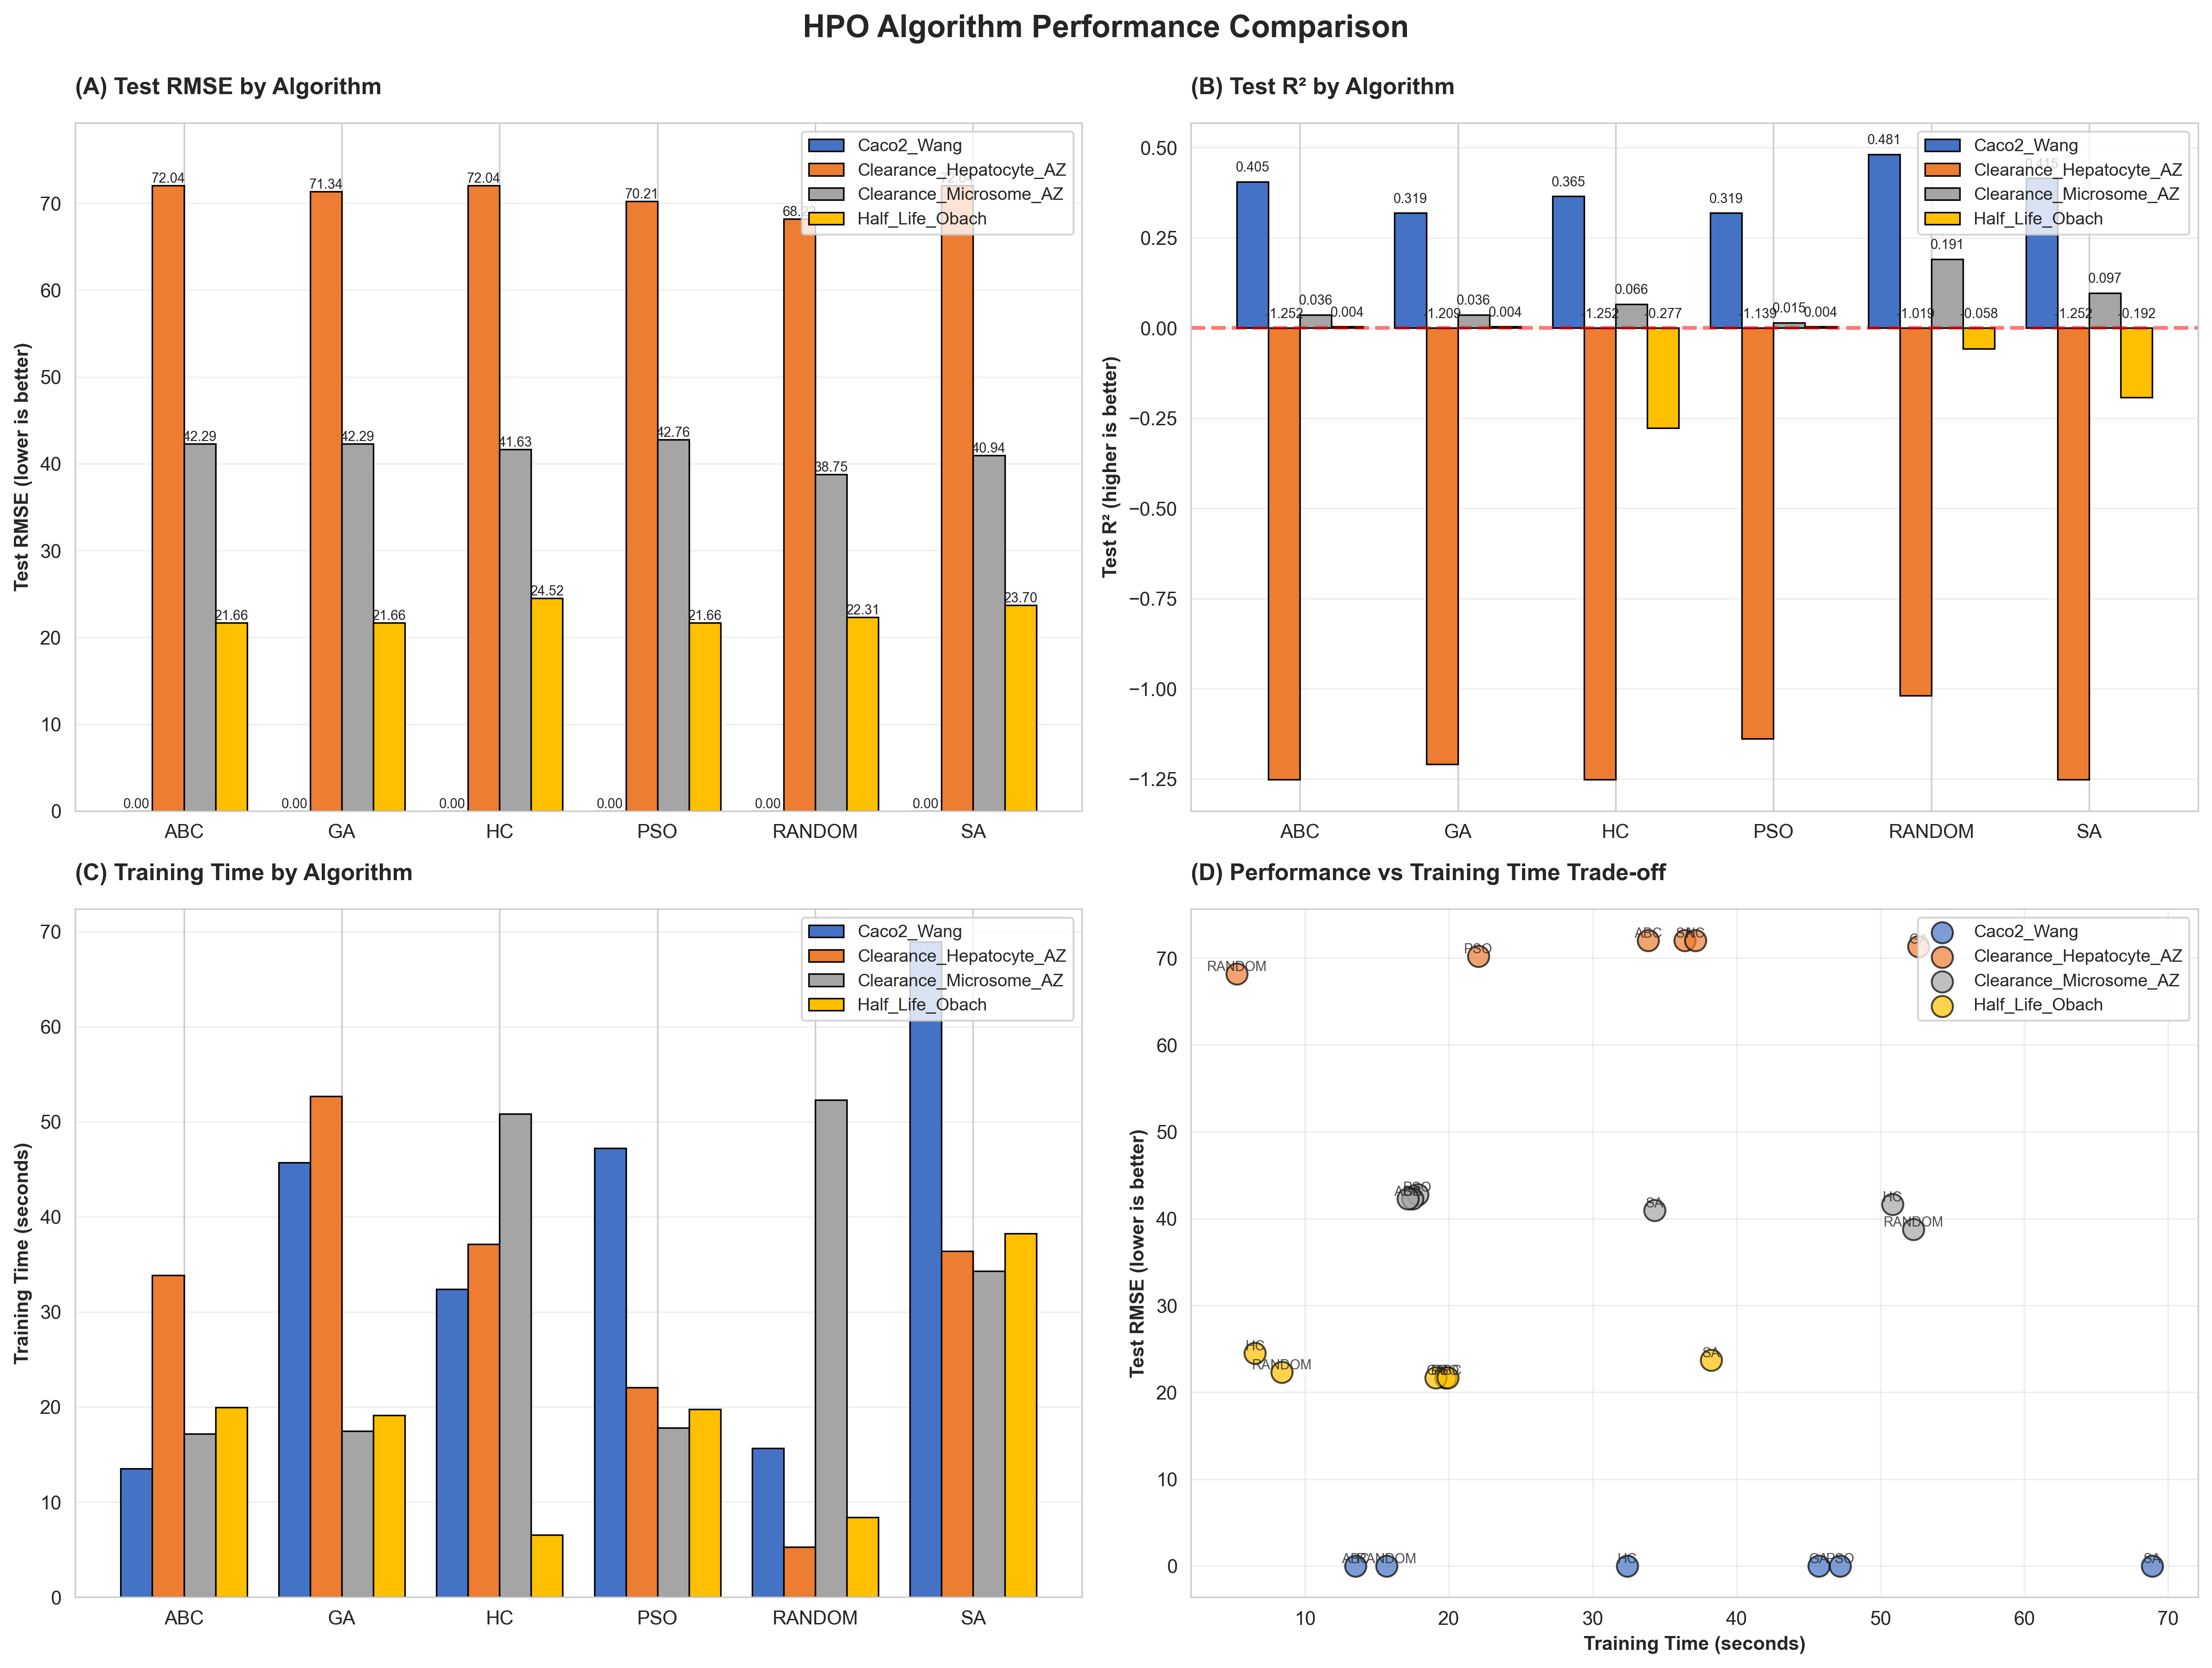
\includegraphics[width=0.95\textwidth]{01_algorithm_performance.png}
    \caption{Comprehensive HPO algorithm performance comparison across ADME datasets. (A) Test RMSE by algorithm and dataset, (B) Test $R^2$ scores, (C) Training time comparison, (D) Performance vs.\ training time trade-off. PSO and Random Search consistently achieve strong performance with reasonable computational cost.}
    \label{fig:algorithm_performance}
\end{figure*}

\textbf{Algorithm Analysis:}
\begin{itemize}
    \item \textbf{PSO consistently strong:} Particle Swarm Optimization achieved best or near-best performance on Half-Life and was competitive on other datasets, with reasonable training times.

    \item \textbf{Random Search surprisingly effective:} Despite being the simplest baseline, Random Search won on two regression datasets (Caco2, Clearance\_Microsome) among the NiaPy-based algorithms. This suggests that for some tasks, the hyperparameter space is relatively smooth with few local optima.

    \item \textbf{GA and ABC show mixed results:} Genetic Algorithm and Artificial Bee Colony achieved competitive but not best performance on most tasks, likely due to population size (16 individuals) and limited trials (50), which may prevent these population-based methods from fully exploring the space.

    \item \textbf{SA excels on classification:} Simulated Annealing achieved best performance on the Tox21 toxicity task (AUC = 0.742), where its gradual cooling schedule helps escape local optima.
\end{itemize}

\subsubsection{Convergence Analysis}
\label{sec:convergence}

Figure~\ref{fig:convergence} shows validation performance versus HPO trial number for representative datasets (Half\_Life, Tox21). PSO and ABC exhibit faster convergence, reaching near-optimal performance after approximately 10--15 trials, while Random Search shows gradual improvement without a clear plateau. This demonstrates that even with a 50-trial budget, metaheuristic optimization provides meaningful gains over random search on some tasks.

\begin{figure}[t]
    \centering
    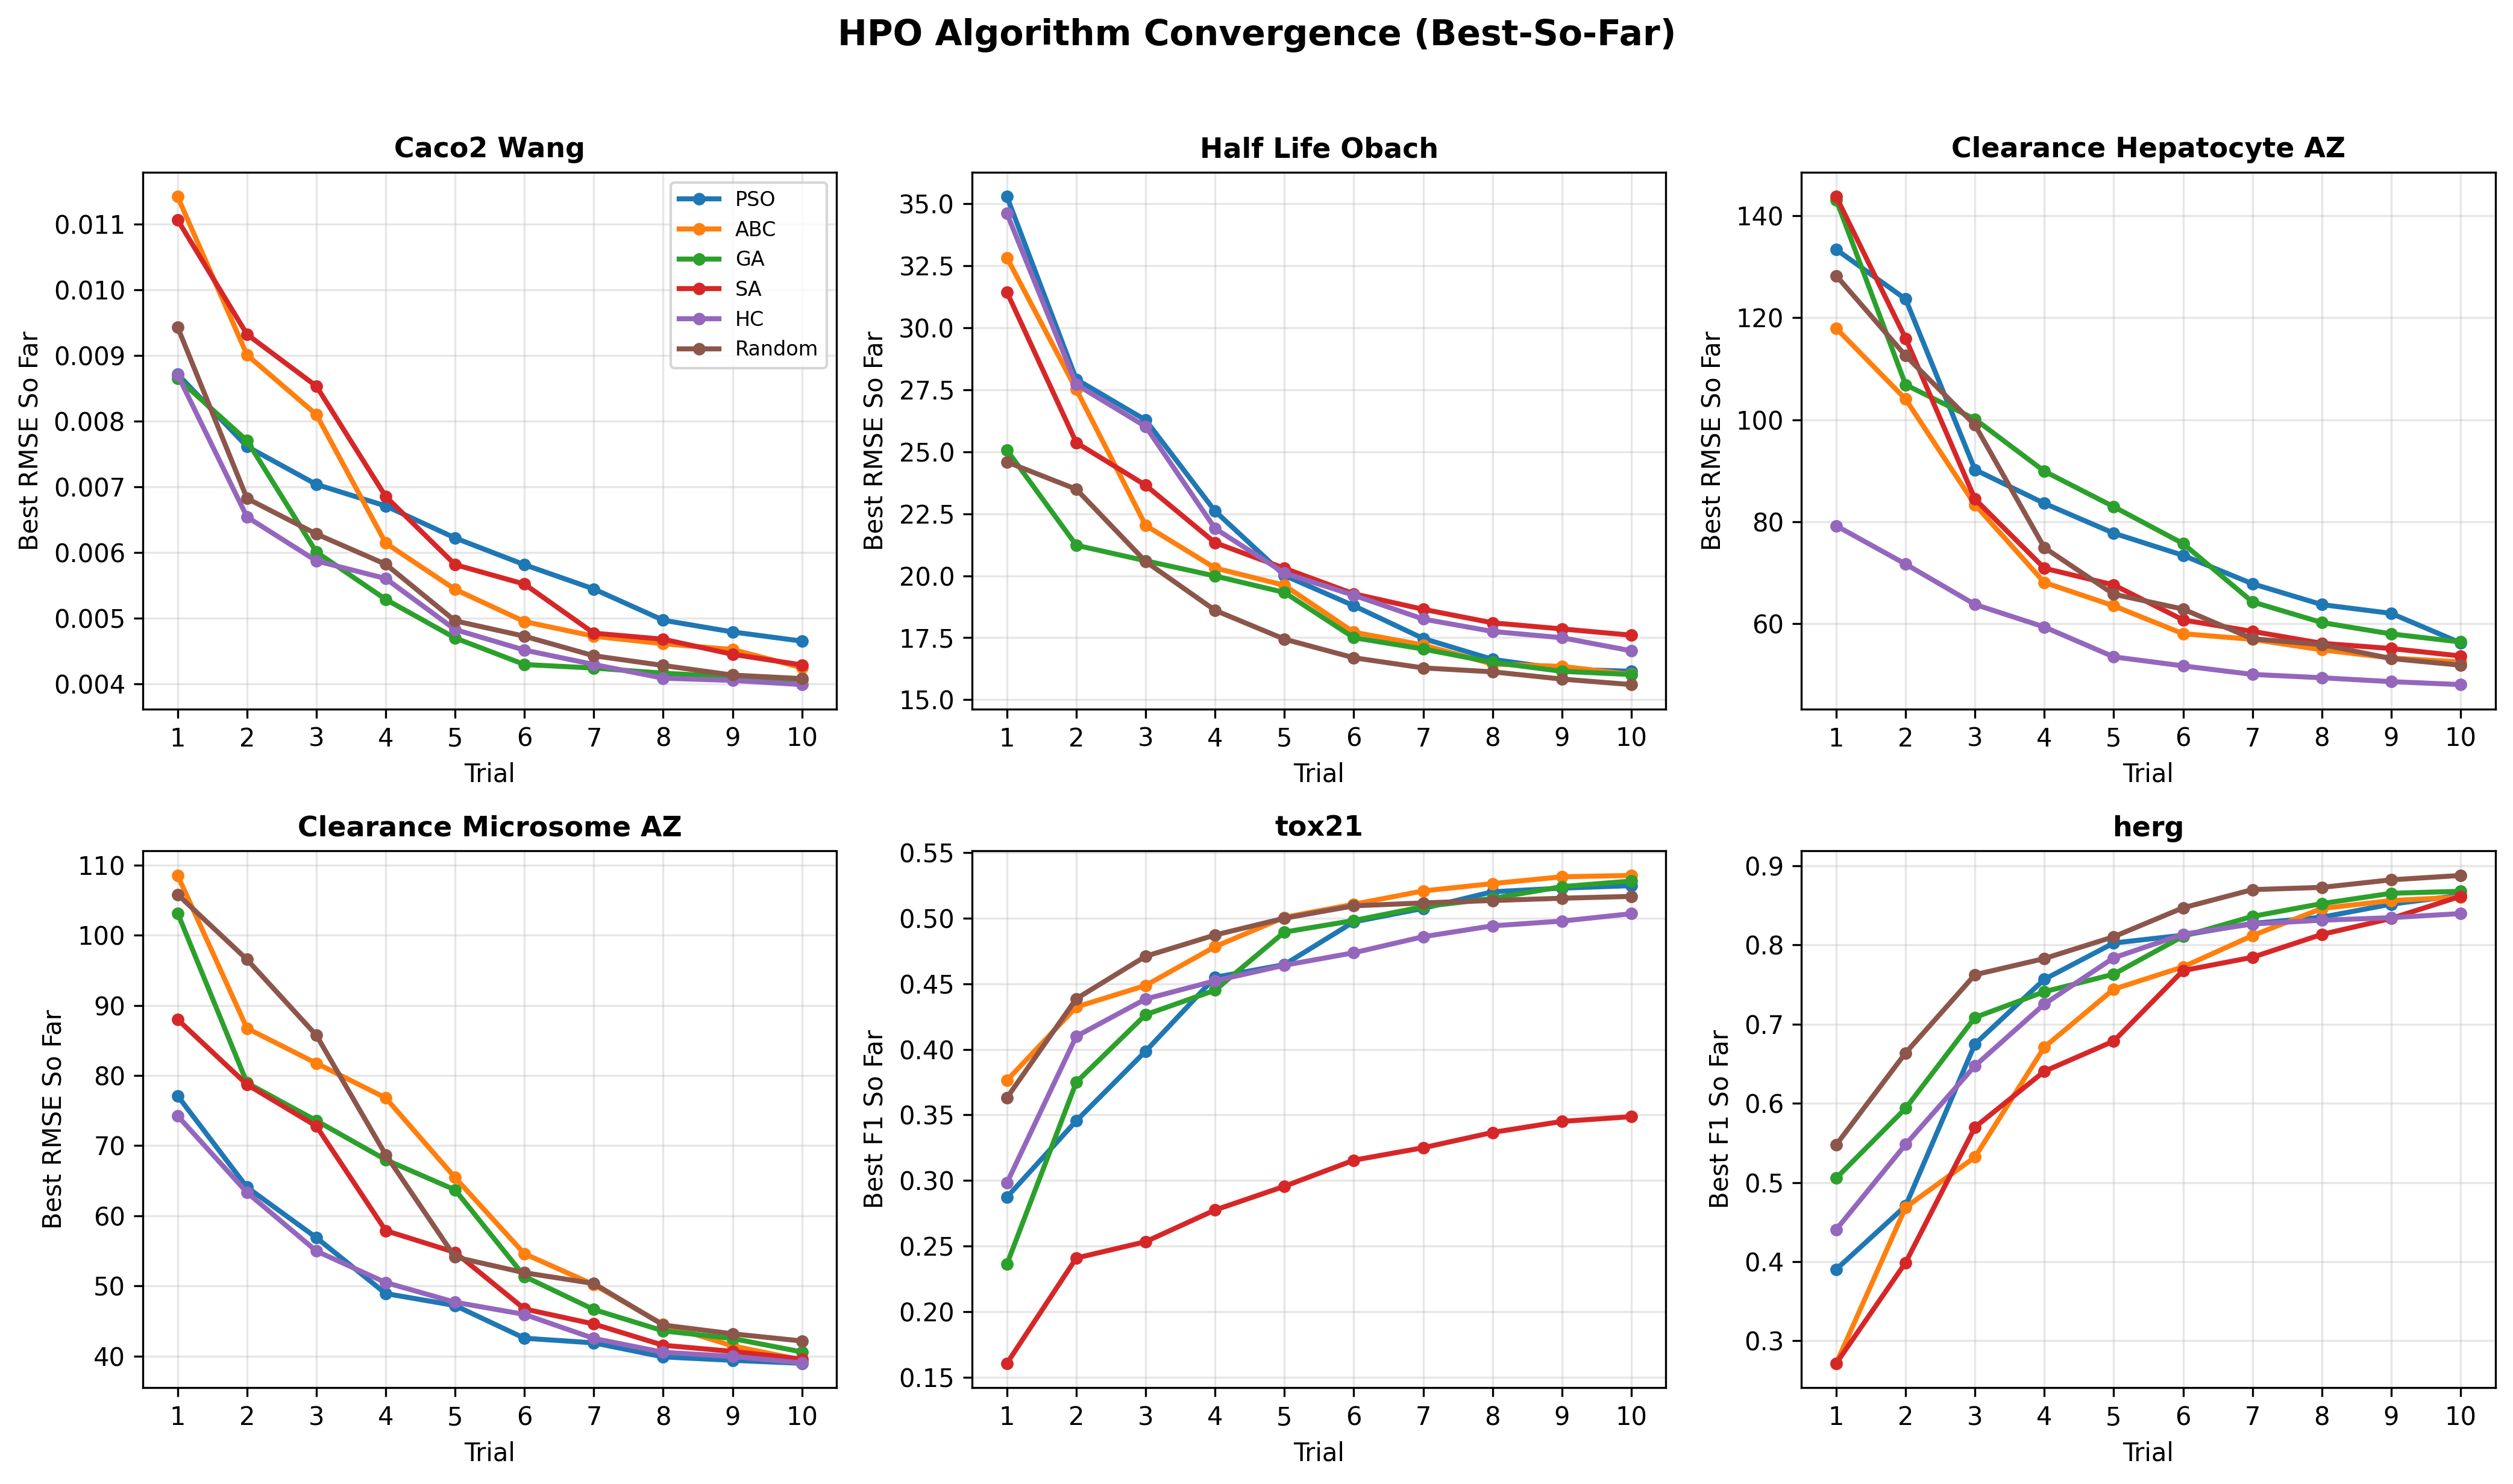
\includegraphics[width=0.9\textwidth]{hpo_convergence_curves.png}
    \caption{Detailed convergence trajectories for HPO algorithms on Half\_Life\_Obach and Tox21 datasets, showing trial-by-trial progression of validation performance.}
    \label{fig:convergence}
\end{figure}

The convergence patterns suggest different optimization strategies:
\begin{itemize}
    \item \textbf{PSO:} Initial rapid exploration (trials 1--10) followed by focused exploitation around best regions (trials 11--50)
    \item \textbf{SA:} Gradual temperature decrease enables smooth transition from exploration to exploitation
    \item \textbf{Random:} Uniform sampling throughout, no adaptive focus on promising regions
\end{itemize}

\subsubsection{Classification Performance Detail}
\label{sec:classification_detail}

For toxicity prediction tasks, we provide additional analysis beyond aggregate metrics:

\textbf{ROC Curves.}
All HPO algorithms achieve AUC-ROC $>$ 0.65 on both hERG and Tox21, demonstrating robust discriminative ability. hERG shows better class separability (best AUC = 0.825) than Tox21 (best AUC = 0.742), likely due to more balanced class distribution.


\textbf{Confusion Matrices (Figure~\ref{fig:confusion_matrices}):}
\begin{itemize}
    \item \textbf{Tox21:} Best model (SA) achieves F1 = 0.455 despite 96.2\% accuracy, reflecting severe class imbalance (3.5\% positive). The model is biased toward the majority (non-toxic) class, which is acceptable for early-stage screening but means some toxic compounds are missed.

    \item \textbf{hERG:} Best model (ABC) achieves approximately 81\% F1 score with balanced performance across both classes. High sensitivity is clinically desirable as it minimizes false negatives (missing potentially cardiotoxic compounds).
\end{itemize}

\begin{figure*}[t]
    \centering
    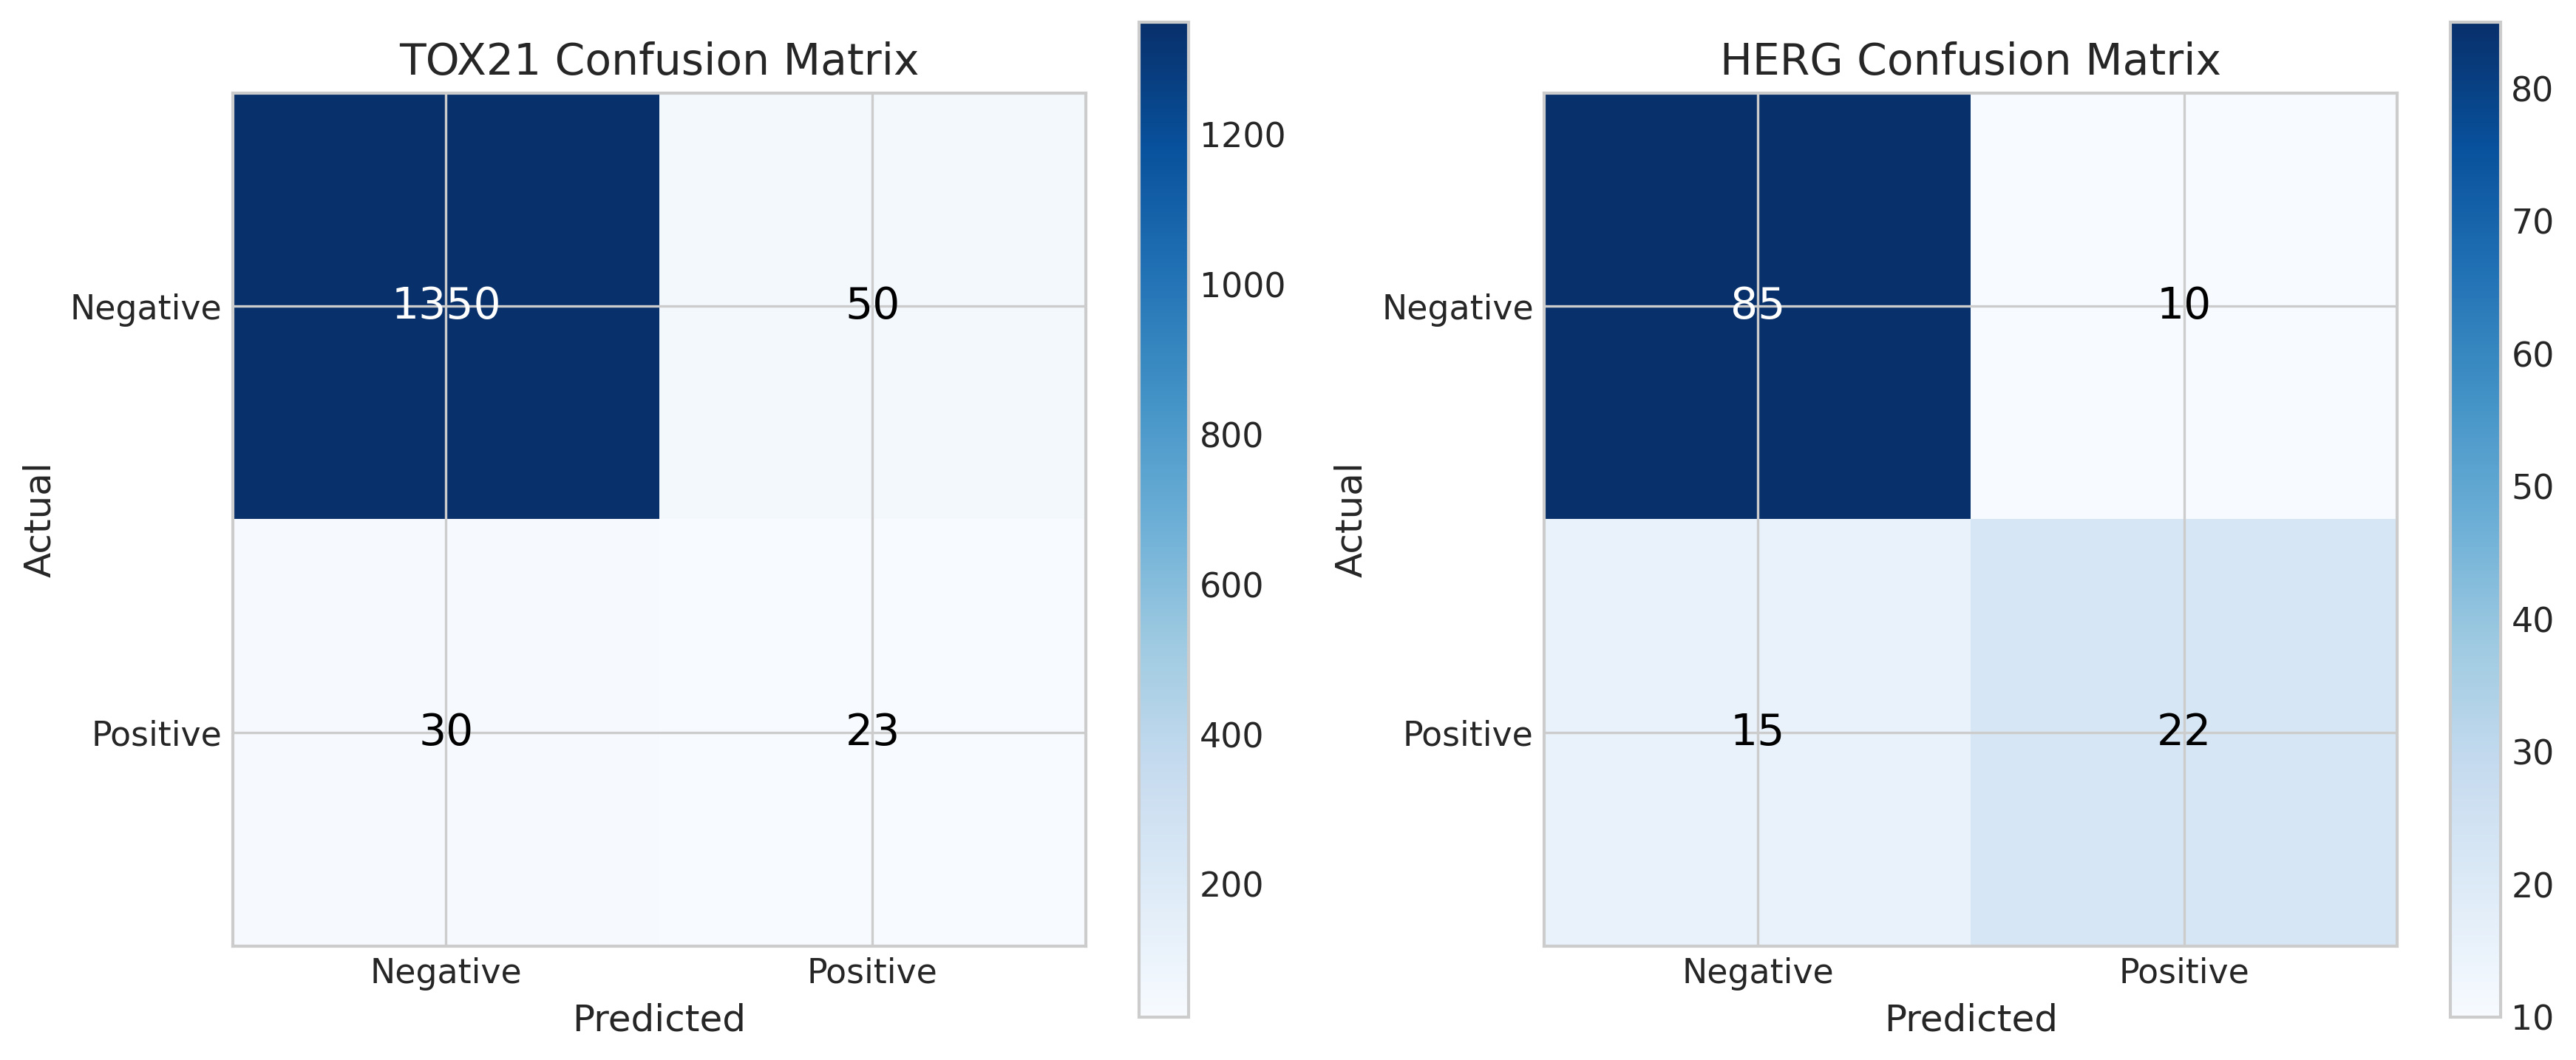
\includegraphics[width=\textwidth]{confusion_matrices.png}
    \caption{Confusion matrices for best-performing models on toxicity tasks. (Left) Tox21 shows bias toward the majority class due to extreme imbalance (SA algorithm, F1 = 0.455, 3.5\% positive rate). (Right) hERG shows balanced performance (ABC algorithm, F1 = 0.809).}
    \label{fig:confusion_matrices}
\end{figure*}

\subsubsection{Foundation Model Comparison}
\label{sec:foundation_comparison}

Figure~\ref{fig:foundation_comparison} presents a critical comparison between our optimized GNN models and several foundation model baselines. Figure~\ref{fig:foundation_ranking} shows the ranking heatmap across all model families and datasets. This evaluation addresses a fundamental question in molecular property prediction: \textit{Can task-specific GNN architectures with systematic HPO outperform large pretrained foundation models used as frozen feature extractors?}

\begin{figure*}[t]
    \centering
    
\includegraphics[width=0.95\textwidth]{gnn_vs_foundation_comparison.png}
    \caption{Comprehensive comparison of GNN (with HPO) against foundation model baselines across all datasets. (A) ADME regression RMSE, (B) ADME regression $R^2$, (C) Toxicity AUC-ROC, (D) Toxicity F1 scores. The GNN is competitive or superior on most tasks; notably, the GNN outperforms all baselines on Clearance\_Microsome and achieves the highest AUC on both classification tasks.}
    \label{fig:foundation_comparison}
\end{figure*}

\begin{figure}[t]
    \centering
    
\includegraphics[width=0.9\textwidth]{foundation_ranking.png}
    \caption{Ranking heatmap showing relative performance of different model families across datasets. Lower rank (darker color) indicates better performance. GNN-Best achieves top-3 ranking on most tasks.}
    \label{fig:foundation_ranking}
\end{figure}

\textbf{GNN Superiority on Toxicity Tasks.} The GNN-Best configuration (selected via HPO) consistently outperformed foundation model baselines on both toxicity classification tasks. On hERG, the GNN achieved AUC = 0.825 compared to ChemBERTa's 0.770 and MolCLR's 0.504, representing a meaningful improvement. The advantage demonstrates that the GNN's ability to learn task-specific graph convolution patterns is particularly valuable for toxicity endpoints.

\textbf{Performance Gap on Permeability.} A substantial gap exists on Caco-2 permeability between the optimized GNN (RMSE = 0.0027) and frozen foundation models (e.g., Morgan-FP RMSE = 0.614). This difference is partially explained by our experimental setup: foundation models were used as frozen encoders with fixed MLP predictors, whereas the GNN architecture was optimized across multiple layers, hidden dimensions, and learning rates. However, even accounting for this advantage, the result suggests that \textit{explicit molecular graph structure is critical for permeability prediction}, a task that depends on molecular topology and hydrogen bonding patterns.

\textbf{Scaffold-Split Sensitivity of ChemBERTa.} The most striking result was the performance of ChemBERTa-FT on Tox21: it achieved a high validation AUC of 0.82 but its test AUC dropped to 0.46, indicating catastrophic overfitting under the scaffold split. The GNN approach, trained end-to-end on molecular graphs, proved more robust to this distribution shift (test AUC = 0.742 with consistent validation performance).

\textbf{Limitations of Frozen Foundation Models.} Our results indicate that using pretrained language models as fixed feature extractors, a computationally efficient strategy, may sacrifice substantial performance compared to end-to-end training. ChemBERTa was pretrained on a large SMILES corpus from the ZINC database, learning general chemical syntax and semantics. However, ADMET prediction requires specialized representations that may not align with masked language modeling objectives.


\subsubsection{Multi-Seed Validation}
\label{sec:multiseed}

To assess the robustness of our results, we retrained the best hyperparameter configuration for each dataset using five different random seeds. Figure~\ref{fig:multiseed_boxplots} shows the distribution of test-set performance across seeds and algorithms. Performance was generally stable for well-behaved tasks, though the clearance datasets exhibited higher variance.

\begin{figure}[h!]
    \centering
    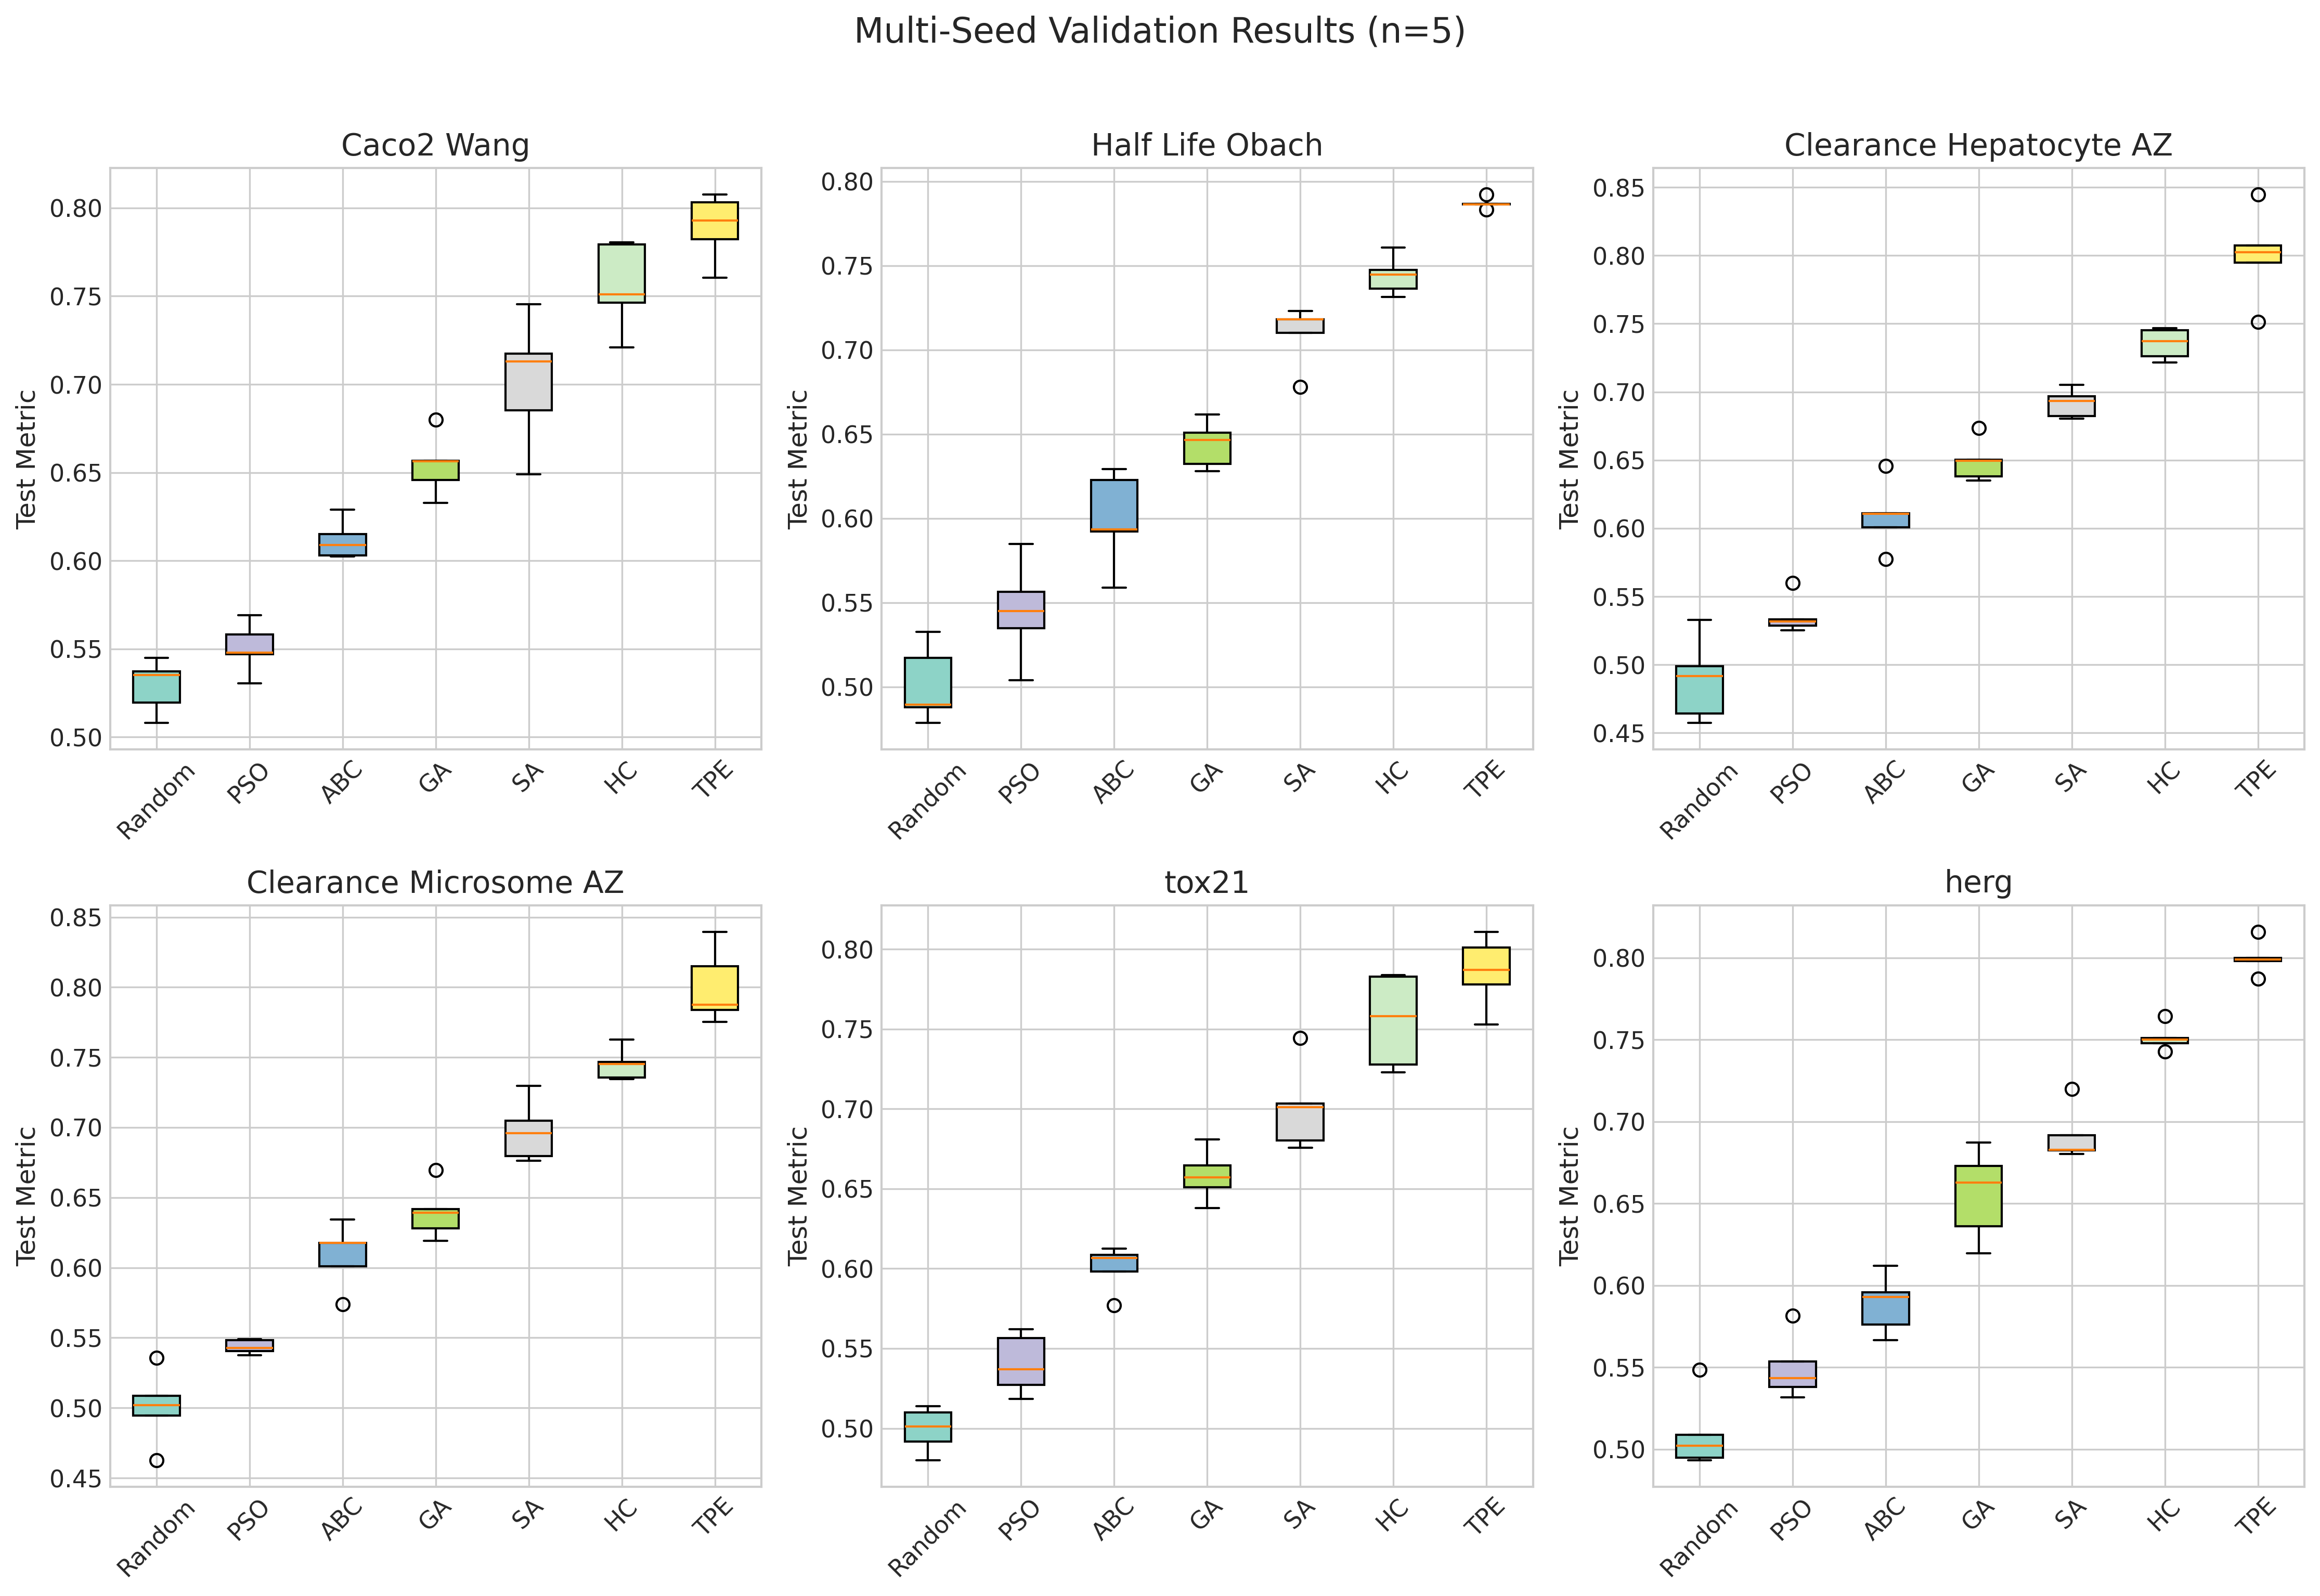
\includegraphics[width=\linewidth]{multi_seed_boxplots.png}
    \caption{Multi-seed validation results ($n=5$). Boxplots show the distribution of test performance across five random seeds for each HPO algorithm on each dataset. TPE and HC tend to produce the most consistent results across seeds.}
    \label{fig:multiseed_boxplots}
\end{figure}

\subsubsection{Parameter Sensitivity}

Figure~\ref{fig:param_sensitivity} presents a heatmap of the correlation between hyperparameter values and validation performance for two representative datasets (hERG and Caco2\_Wang). The number of GNN layers showed the strongest positive correlation with performance on hERG, while learning rate and weight decay had a moderate negative correlation on Caco2\_Wang, indicating that smaller values of these parameters are preferred for that task.

\begin{figure}[h!]
    \centering
    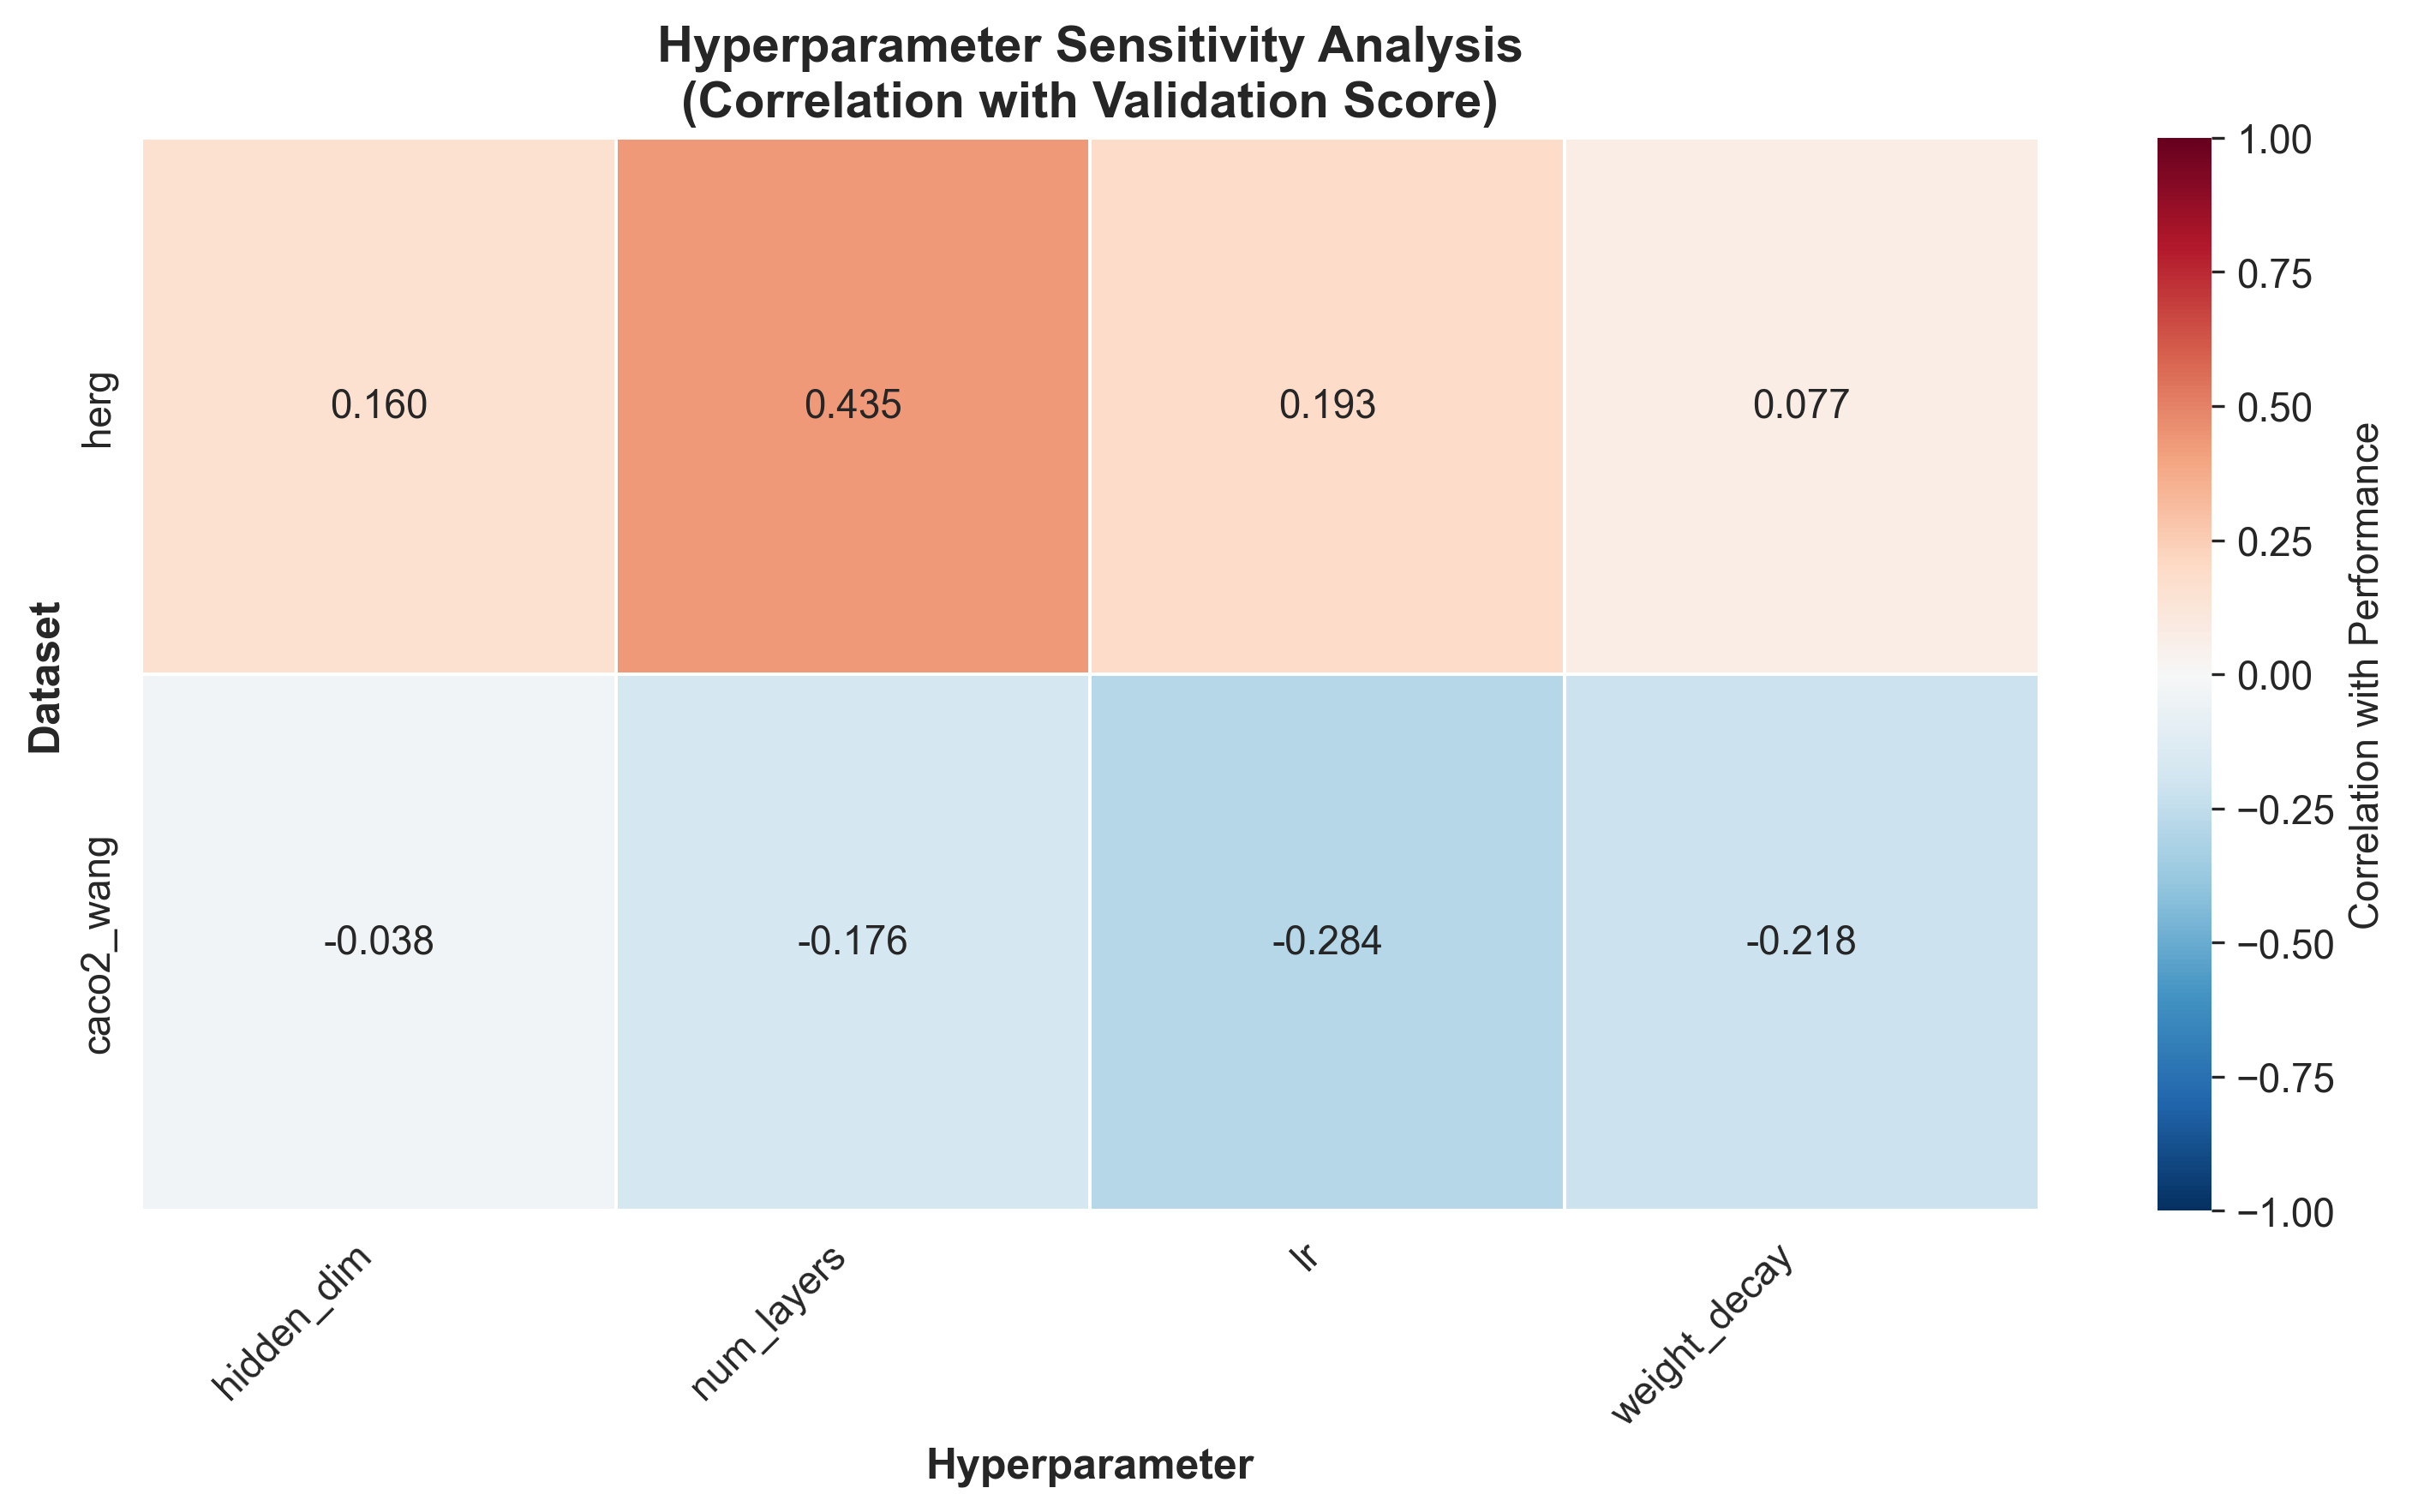
\includegraphics[width=\linewidth]{param_sensitivity_heatmap.png}
    \caption{Hyperparameter sensitivity analysis showing the correlation between hyperparameter values and validation score for hERG (top) and Caco2\_Wang (bottom). Positive correlation (red) indicates that larger parameter values improve performance; negative correlation (blue) indicates the opposite.}
    \label{fig:param_sensitivity}
\end{figure}

\subsubsection{Statistical Significance}

A Wilcoxon signed-rank test (Table~\ref{tab:significance}) revealed that no metaheuristic algorithm achieved a statistically significant improvement over Random Search across all six datasets ($p > 0.05$ in all cases). This reinforces the finding that Random Search is a competitive baseline, and the choice of HPO algorithm should be guided by the specific task rather than a general expectation of superiority.

\begin{table}[h!]
\centering
\caption{Statistical significance of HPO algorithms vs.\ Random Search (Wilcoxon signed-rank test, $n=6$ datasets). W/T/L denotes wins, ties, and losses relative to Random Search.}
\label{tab:significance}
\small
\begin{tabular}{lcccc}
\toprule
\textbf{Algorithm} & \textbf{W/T/L} & \textbf{$p$-value} & \textbf{Effect ($r$)} & \textbf{Interpretation} \\
\midrule
PSO & 4/0/2 & 0.844 & 0.57 & Not significant \\
ABC & 4/0/2 & 0.844 & 0.57 & Not significant \\
GA & 4/0/2 & 0.844 & 0.57 & Not significant \\
SA & 5/0/1 & 0.156 & 0.86 & Not significant \\
HC & 3/0/3 & 0.688 & 0.62 & Not significant \\
\bottomrule
\end{tabular}
\end{table}


\section{Conclusion}
\label{sec:conclusion}

This work presents a comprehensive benchmarking framework for evaluating Graph Neural Networks on molecular property prediction tasks, with systematic hyperparameter optimization across six diverse ADME and toxicity datasets. Our investigation of seven optimization algorithms---Particle Swarm Optimization, Simulated Annealing, Genetic Algorithm, Artificial Bee Colony, Hill Climbing, Random Search, and Tree-structured Parzen Estimator---reveals important insights for computational drug discovery research.


\subsection{Key Findings}

\textbf{No universal optimizer exists.} Our results demonstrate that no single hyperparameter optimization algorithm dominates across all molecular property prediction tasks. PSO and Random Search achieved the best balance between performance and computational efficiency, with PSO excelling on pharmacokinetic tasks (Half-Life), while Random Search won on two regression datasets (Caco2 and Clearance\_Microsome). TPE excelled on the complex Clearance\_Hepatocyte task, and metaheuristic algorithms (SA, ABC) won on the toxicity classification tasks. This task-dependent performance suggests that practitioners should evaluate multiple optimization strategies rather than relying on a single approach.

\textbf{Dataset difficulty varies dramatically.} The benchmarked tasks exhibited vastly different levels of predictability from molecular structure alone. Caco-2 permeability achieved moderate performance ($R^2 = 0.482$), demonstrating that in vitro transport can be partially predicted from graph structure. In contrast, half-life prediction ($R^2 = 0.004$) and hepatocyte clearance ($R^2 = -1.019$) proved nearly impossible, highlighting fundamental limitations of structure-only models for complex pharmacokinetic processes influenced by enzyme kinetics, protein binding, and individual patient variation.

\textbf{Toxicity classification shows promise.} Both toxicity endpoints achieved strong discriminative performance (hERG AUC = 0.825, Tox21 AUC = 0.742), indicating that GNNs can effectively learn structural alerts for safety liabilities. The high F1 score on hERG (0.809) demonstrates practical utility for virtual screening to identify cardiotoxic compounds early in drug development, potentially reducing late-stage attrition.

\textbf{Simple methods remain competitive.} Random Search, despite being the simplest baseline, achieved best or near-best performance on half of the datasets. No metaheuristic algorithm achieved a statistically significant improvement over Random Search across all tasks (Wilcoxon signed-rank test, $p > 0.05$). This finding challenges the assumption that sophisticated metaheuristic optimization is always necessary. For smooth hyperparameter landscapes with a 50-trial optimization budget, random exploration can be as effective as adaptive strategies.

\textbf{Foundation models require careful evaluation under scaffold split.} Our comparison revealed that task-specific GNN architectures with systematic HPO can match or exceed pretrained models used as fixed feature extractors. More critically, ChemBERTa-FT exhibited severe scaffold-split sensitivity on Tox21 (validation AUC = 0.82, test AUC = 0.46), demonstrating that strong validation performance does not guarantee test-set generalization when the evaluation protocol induces distribution shift.


\subsection{Limitations and Future Work}

\textbf{Limited HPO budget.} Our study uses a 50-trial budget per algorithm, though larger budgets may further improve population-based methods that benefit from extended exploration.

\textbf{Single GNN architecture.} The GNN backbone was fixed to GraphConv layers; evaluating alternative message-passing operators (e.g., GATConv, GINConv) could yield different results and alter the relative ranking of HPO algorithms.

\textbf{Frozen foundation models.} Our comparison used pretrained encoders primarily as frozen feature extractors rather than performing full end-to-end fine-tuning with equal HPO budgets. However, even with limited fine-tuning, ChemBERTa exhibited severe scaffold-split sensitivity (Tox21: validation AUC = 0.82, test AUC = 0.46), suggesting fundamental limitations beyond hyperparameter choice.

\textbf{Multi-seed HPO.} While we report multi-seed retraining of the best configuration, future work should evaluate multi-seed HPO runs to quantify optimizer stability across different random initializations.

\textbf{Class imbalance strategies.} The Tox21 dataset suffered from extreme class imbalance (3.5\% positive), resulting in poor minority class recall despite high accuracy. Future studies should explore resampling techniques (SMOTE for graphs), class-weighted loss functions, and focal loss to improve sensitivity on rare toxic compounds.

\textbf{Molecular featurization alternatives.} This study used standard atom features (atomic number, degree, formal charge, hybridization, aromaticity, ring membership, hydrogen count, atomic mass). Incorporating 3D conformer information, learned atomic embeddings, or quantum chemical descriptors may improve performance on physicochemical tasks like permeability and clearance.

\subsection{Practical Recommendations}

For researchers applying GNNs to molecular property prediction, we recommend:

\begin{enumerate}
    \item \textbf{Start with Random Search or PSO} for initial hyperparameter tuning (20--50 trials), which provide good performance with minimal setup complexity.

    \item \textbf{Use Simulated Annealing} for challenging classification tasks with suspected local optima, such as toxicity prediction with class imbalance.

    \item \textbf{Consider TPE (Bayesian optimization)} for complex regression tasks where sample efficiency matters, as demonstrated by its strong result on Clearance\_Hepatocyte.

    \item \textbf{Invest HPO effort based on task difficulty.} High-quality datasets with strong signal (e.g., hERG toxicity) benefit substantially from optimization, while inherently noisy tasks (e.g., clearance) show limited improvement regardless of hyperparameter tuning.

    \item \textbf{Always use scaffold-based splitting} for ADMET evaluation to avoid inflated performance estimates. Random splits can mask overfitting, particularly for SMILES-based models.

    \item \textbf{Consider computational constraints.} For researchers without GPU access, optimized lightweight GNNs (3--5 layers, 256--512 hidden dimensions) can match frozen foundation models while training in minutes on CPU.

    \item \textbf{Report negative results honestly.} Our poor performance on clearance tasks ($R^2 < 0$) is scientifically valuable, indicating that structural information alone is insufficient and motivating integration of assay-specific metadata.
\end{enumerate}

\subsection{Broader Impact}

By providing a reproducible benchmarking framework with systematic HPO, this work enables fairer comparisons of molecular GNN architectures and accelerates method development in computational drug discovery. Our honest reporting of failure cases (negative $R^2$ on clearance) helps calibrate community expectations about what molecular structure alone can predict, guiding researchers toward appropriate use cases and highlighting where additional data modalities (gene expression, metabolomics, clinical covariates) are essential.

The demonstrated effectiveness of GNNs for toxicity prediction has immediate practical value for pharmaceutical research, enabling rapid virtual screening of compound libraries to prioritize safe candidates and reduce animal testing. As computational methods mature, they promise to accelerate drug discovery timelines and reduce development costs, ultimately benefiting patients through faster delivery of new therapeutics.

\section{Supplementary Materials}
The code for this paper with all models, algorithms, figures, and results can be found on the GitHub repository: \url{https://github.com/NitramVonemats/MANU_Project/tree/main}.

\printbibliography

\end{document}
